\chapter{Rigid Multibody Dynamics}
\label{chp:back_RBDynamics}

In this chapter, a mathematical groundwork for characterizing the dynamics of a floating-base multibody system is presented, setting a convention that is used throughout this work. Then, a first introduction to recursive algorithm for the computation of the dynamics of a multibody system is presented, to give a comprehensive understanding of the state of the art in the field of rigid multibody dynamics algorithms. In the forthcoming discussion, a 6D \textit{spatial vectors} notation firstly introduced by \citet{featherstone_rigid_2008} and successively integrated and adapted by \citet{traversaro_multibody_2019} is presented. As a matter of fact, this notation allows to describe the motion of a rigid body without excessive use of indices, which can be confusing and error-prone when dealing with complex recursive algorithms that will be further discussed. This convention will be used to describe the kinematics and dynamics of a floating-base multibody system in a unified manner throughout this work.

\section{Formalisms and Notation}

\paragraph{Spatial Vectors} A spatial vector is a 6D vector that describes the motion of a rigid body in space.

In the case of a rigid body, the velocity of a point $O$ attached to the body with respect to a reference frame attached to an arbitrary point $O$ in the space can be generally expressed by its angular component $\mathbf{\omega}$ about an axis passing through $O$ and its linear component $\mathbf{v} _A$, for which the following relation holds:

\begin{equation}
    v _A = \mathbf{\omega} \times \bar{OP}
\end{equation}

where $\bar{OP}$ is the position vector of $P$ with respect to $O$. This holds for any point $O$ on the rigid body. In order to simplify the notation, introducing a Cartesian coordinate frame $\mathcal{O} _{xyz}$, we can define a basis of 6 spatial vectors $\mathcal{D} _O = \{\mathbf{d} _i\} ^6 _{i=1}$ as:

\begin{equation}
    \mathcal{D} _O = \{\mathbf{d} _x, \mathbf{d} _y, \mathbf{d} _z, \mathbf{d} _{O _x}, \mathbf{d} _{O _y}, \mathbf{d} _{O _z} \} \subset \mathcal{M} ^6
\end{equation}

where $\mathcal{M} ^6$ is the space of 6D vectors, defining a Pl\"ucker coordinate system on $\mathcal{M} ^6$ as shown in \cref{fig:pluecker}.

% === Fig: Pluecker === %
\begin{figure}
    \centering
    \caption{Pl\"ucker motion coordinate system}
    \label{fig:pluecker}
    \tikzset{every picture/.style={line width=0.75pt}}
    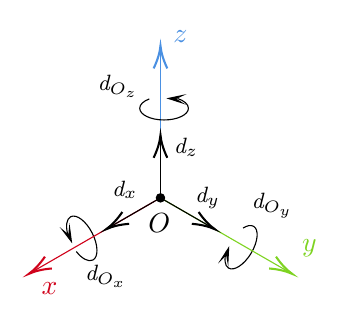
\begin{tikzpicture}[x=0.75pt,y=0.75pt,yscale=-1,xscale=1]
        \draw [color={rgb, 255:red, 74; green, 144; blue, 226 }  ,draw opacity=1 ]   (249.79,80.38) -- (249.79,9.08) ;
        \draw [shift={(249.79,7.08)}, rotate = 90] [color={rgb, 255:red, 74; green, 144; blue, 226 }  ,draw opacity=1 ][line width=0.75]    (10.93,-3.29) .. controls (6.95,-1.4) and (3.31,-0.3) .. (0,0) .. controls (3.31,0.3) and (6.95,1.4) .. (10.93,3.29)   ;
        \draw  [draw opacity=0] (257.99,32.5) .. controls (261.16,33.51) and (263.25,35.24) .. (263.25,37.21) .. controls (263.25,40.32) and (258,42.85) .. (251.52,42.85) .. controls (245.05,42.85) and (239.8,40.32) .. (239.8,37.21) .. controls (239.8,35.38) and (241.61,33.75) .. (244.41,32.72) -- (251.52,37.21) -- cycle ; \draw   (257.99,32.5) .. controls (261.16,33.51) and (263.25,35.24) .. (263.25,37.21) .. controls (263.25,40.32) and (258,42.85) .. (251.52,42.85) .. controls (245.05,42.85) and (239.8,40.32) .. (239.8,37.21) .. controls (239.8,35.38) and (241.61,33.75) .. (244.41,32.72) ;
        \draw  [draw opacity=0] (205.05,97.73) .. controls (204.06,93.79) and (204.55,90.48) .. (206.55,89.46) .. controls (209.33,88.05) and (213.96,91.58) .. (216.9,97.35) .. controls (219.84,103.12) and (219.97,108.94) .. (217.19,110.35) .. controls (215.09,111.42) and (211.93,109.66) .. (209.25,106.25) -- (211.87,99.91) -- cycle ; \draw   (205.05,97.73) .. controls (204.06,93.79) and (204.55,90.48) .. (206.55,89.46) .. controls (209.33,88.05) and (213.96,91.58) .. (216.9,97.35) .. controls (219.84,103.12) and (219.97,108.94) .. (217.19,110.35) .. controls (215.09,111.42) and (211.93,109.66) .. (209.25,106.25) ;
        \draw  [draw opacity=0] (289.6,94.92) .. controls (291.53,93.69) and (293.37,93.33) .. (294.68,94.12) .. controls (297.34,95.72) and (296.8,101.52) .. (293.45,107.07) .. controls (290.11,112.61) and (285.24,115.81) .. (282.57,114.2) .. controls (280.67,113.05) and (280.4,109.78) .. (281.61,105.98) -- (288.62,104.16) -- cycle ; \draw   (289.6,94.92) .. controls (291.53,93.69) and (293.37,93.33) .. (294.68,94.12) .. controls (297.34,95.72) and (296.8,101.52) .. (293.45,107.07) .. controls (290.11,112.61) and (285.24,115.81) .. (282.57,114.2) .. controls (280.67,113.05) and (280.4,109.78) .. (281.61,105.98) ;
        \draw  [fill={rgb, 255:red, 0; green, 0; blue, 0 }  ,fill opacity=1 ] (205.98,94.78) -- (206.86,101.37) -- (202.81,96.09) -- (205.63,98.4) -- cycle ;
        \draw  [fill={rgb, 255:red, 0; green, 0; blue, 0 }  ,fill opacity=1 ] (279.01,110.18) -- (282.61,104.59) -- (282.28,111.23) -- (281.63,107.65) -- cycle ;
        \draw  [fill={rgb, 255:red, 0; green, 0; blue, 0 }  ,fill opacity=1 ] (260,34.53) -- (253.67,32.48) -- (260.18,31.11) -- (256.88,32.65) -- cycle ;
        \draw [color={rgb, 255:red, 126; green, 211; blue, 33 }  ,draw opacity=1 ]   (249.79,80.38) -- (311.53,116.02) ;
        \draw [shift={(313.27,117.02)}, rotate = 210] [color={rgb, 255:red, 126; green, 211; blue, 33 }  ,draw opacity=1 ][line width=0.75]    (10.93,-3.29) .. controls (6.95,-1.4) and (3.31,-0.3) .. (0,0) .. controls (3.31,0.3) and (6.95,1.4) .. (10.93,3.29)   ;
        \draw [color={rgb, 255:red, 208; green, 2; blue, 27 }  ,draw opacity=1 ]   (249.79,80.37) -- (218.61,98.38) -- (188.04,116.02) ;
        \draw [shift={(186.31,117.02)}, rotate = 330] [color={rgb, 255:red, 208; green, 2; blue, 27 }  ,draw opacity=1 ][line width=0.75]    (10.93,-3.29) .. controls (6.95,-1.4) and (3.31,-0.3) .. (0,0) .. controls (3.31,0.3) and (6.95,1.4) .. (10.93,3.29)   ;
        \draw    (249.79,80.38) -- (249.79,52.13) ;
        \draw [shift={(249.79,50.13)}, rotate = 90] [color={rgb, 255:red, 0; green, 0; blue, 0 }  ][line width=0.75]    (10.93,-3.29) .. controls (6.95,-1.4) and (3.31,-0.3) .. (0,0) .. controls (3.31,0.3) and (6.95,1.4) .. (10.93,3.29)   ;
        \draw    (249.79,80.38) -- (274.25,94.5) ;
        \draw [shift={(275.99,95.5)}, rotate = 210] [color={rgb, 255:red, 0; green, 0; blue, 0 }  ][line width=0.75]    (10.93,-3.29) .. controls (6.95,-1.4) and (3.31,-0.3) .. (0,0) .. controls (3.31,0.3) and (6.95,1.4) .. (10.93,3.29)   ;
        \draw    (249.79,80.37) -- (225.32,94.5) ;
        \draw [shift={(223.59,95.5)}, rotate = 330] [color={rgb, 255:red, 0; green, 0; blue, 0 }  ][line width=0.75]    (10.93,-3.29) .. controls (6.95,-1.4) and (3.31,-0.3) .. (0,0) .. controls (3.31,0.3) and (6.95,1.4) .. (10.93,3.29)   ;
        \draw (191.23,119.9) node [anchor=north west][inner sep=0.75pt]  [color={rgb, 255:red, 208; green, 2; blue, 27 }  ,opacity=1 ]  {$x$};
        \draw (316.73,99.4) node [anchor=north west][inner sep=0.75pt]  [color={rgb, 255:red, 126; green, 211; blue, 33 }  ,opacity=1 ]  {$y$};
        \draw (254.73,-1.35) node [anchor=north west][inner sep=0.75pt]  [color={rgb, 255:red, 74; green, 144; blue, 226 }  ,opacity=1 ]  {$z$};
        \draw (212.25,111.65) node [anchor=north west][inner sep=0.75pt]  [font=\footnotesize]  {$\mathit{d}_{O_{x}}$};
        \draw (218.25,20.15) node [anchor=north west][inner sep=0.75pt]  [font=\footnotesize]  {$\mathit{d}_{O_{z}}$};
        \draw (292.5,76.9) node [anchor=north west][inner sep=0.75pt]  [font=\footnotesize]  {$\mathit{d}_{O_{y}}$};
        \draw (255,50.4) node [anchor=north west][inner sep=0.75pt]  [font=\footnotesize]  {$\mathit{d}_{z}$};
        \draw (225.25,70.9) node [anchor=north west][inner sep=0.75pt]  [font=\footnotesize]  {$\mathit{d}_{x}$};
        \draw (265.25,73.9) node [anchor=north west][inner sep=0.75pt]  [font=\footnotesize]  {$\mathit{d}_{y}$};
        \draw (242.75,86.65) node [anchor=north west][inner sep=0.75pt]    {$O$};
        \draw [fill={rgb, 255:red, 0; green, 0; blue, 0 }  ,fill opacity=1 ]  (249.79, 80.38) circle [x radius= 2, y radius= 2]   ;
    \end{tikzpicture}
\end{figure}

\paragraph{Spatial Subspace} Once defined $\mathcal{M} ^n$ as a vector space, we can define a subset $\mathrm{S} \subset \mathcal{M} ^n$, which is also a vector space. It can be defined as
the null space of a constraint matrix $\mathbf{K}$, e.g. let $\mathbf{K} \in \mathbb{R} ^{m \times n}$ be a constraint matrix as:

\begin{equation}
    \mathbf{K} = \{ [\mathbf{k} _1, \dots, \mathbf{k} _n]  \subset \mathcal{M} ^m \mid \mathbf{K} \boldsymbol{\nu} = 0 \} \quad \text{with } \mathbf{k} _i \in \mathcal{M} ^m
\end{equation}

we can define the subspace $\mathrm{S}$ as:

\begin{equation}
    \mathrm{S} = \ker (\mathbf{K})
\end{equation}

This defines a motion subspace for a system, e.g. defines the directions in which the system is free to move.

\paragraph{Spatial Velocity} The spatial velocity of a rigid body is defined as a serialization of the linear and angular velocity of a point $A$ attached to the body. In particular, let $\mathbf{p} _A \in \mathcal{D}_O$ be the position vector of $A$ with respect to $O$, then the spatial velocity of the body is defined as the component-wise derivative of the position vector respect to time:

\begin{equation}
    \boldsymbol{\nu} _A = \frac{d}{dt} {}^O\mathbf{p} _A =
    \lim _{\delta t \to 0} \frac{1}{\delta t}
    \begin{bmatrix}
        p _{A _x} (t + \delta t)     & - & p _{A _x} (t) \\
        p _{A _y} (t + \delta t)     & - & p _{A _y} (t) \\
        p _{A _z} (t + \delta t)     & - & p _{A _z} (t) \\
        p _{A _{O_x}} (t + \delta t) & - & p _{A _x} (t) \\
        p _{A _{O_y}} (t + \delta t) & - & p _{A _y} (t) \\
        p _{A _{O_z}} (t + \delta t) & - & p _{A _z} (t) \\
    \end{bmatrix}
    = \begin{bmatrix}
        \mathbf{v} _A \\
        \boldsymbol{\omega} _A
    \end{bmatrix}
\end{equation}

where $\mathbf{v} _A$ is the linear velocity of the point $O$ and $\boldsymbol{\omega} _A$ is the angular velocity of the body.

\paragraph{Spatial Acceleration} Given that the spatial velocity decouples the linear and angular components of the motion, defining a property of the body as a whole and not of a single body-fixed point, the spatial acceleration of a rigid body is defined as simply as just the time derivative of its spatial velocity:

\begin{equation}
    \dot{\boldsymbol{\nu} _A} = \frac{\mathrm{d}}{\mathrm{d}t} \begin{bmatrix}
        \mathbf{v} _A (t) \\
        \boldsymbol{\omega} _A (t)
    \end{bmatrix}
    =
    \begin{bmatrix}
        \dot{\mathbf{v}} _A \\
        \dot{\boldsymbol{\omega}} _A
    \end{bmatrix}
\end{equation}

\paragraph{Spatial Forces} The spatial force acting on a rigid body is defined, in a similar manner as the spatial velocity as a serialization of the linear and the angular components of the wrench acting on the body, in particular, it is related to its motion as:

\begin{equation}
    \mathbf{f} = \begin{bmatrix}
        \mathbf{f} \\
        \boldsymbol{\tau}
    \end{bmatrix} = \mathbf{M}_i \dot{\boldsymbol{\nu}} _i + \boldsymbol{\nu}_i \times ^* \mathbf{M}_i \boldsymbol{\nu}_i
\end{equation}

where $\dot{\boldsymbol{\nu}} \in \mathbb{R}^6$ is the spatial acceleration of the body, $\mathbf{M}_i \in \mathbb{R}^{6 \times 6}$ is the spatial inertia matrix of the body and $\boldsymbol{\nu}_i \in \mathbb{R}^6$ is its spatial velocity.

\section{Kinematics}

\subsection{Joints and Links}

A multibody kinematic tree can be described as a contiguous assembly of two main physical elements: links and joints. The links correspond to the rigid bodies composing the inertial properties of the system, while the joints are usually modeled as massless elements connecting two links, allowing relative motion between them. They are classified according to the number of \ac{DoF} they allow, which is the number of independent coordinates needed to describe the relative motion between the two links, usually assuming values between 0 (fixed joint) and 6 (free joint).

For the sake of simplicity and without loss of generality, in this work, only 1-\ac{DoF} joint will be considered, as their properties can be easily extended to multidimensional cases. In this case, if we recall the definition of the spatial subspace, we can define the joint motion subspace $\mathrm{S} _j \in \mathcal{M} ^6$ as:

\begin{equation}
    \mathrm{S} _j =
    \begin{cases}
        [0, 0, 0, 0, 0, 0] ^\top & \text{if the joint is fixed}     \\
        [0, 0, 1, 0, 0, 0] ^\top & \text{if the joint is prismatic} \\
        [0, 0, 0, 1, 0, 0] ^\top & \text{if the joint is revolute}
    \end{cases}
\end{equation}

\section{Equation of Motion}
\label{sec:back_eom}

The equation of motion of a generic multibody system can be derived starting from the Principle of Least Action, which states that in a time interval $[t _0, t _1]$ the motion of a system is such that the action functional $\mathcal{A}$ is stationary, i.e. the first variation of the action functional is zero:

\begin{equation}
    \mathcal{A} = \int _{t _0} ^{t _1} \mathcal{L} (\mathbf{q}(t), \mathbf{\dot{q}}(t)) dt \quad \text{with } \delta \mathcal{A} = 0
\end{equation}

where $\mathcal{L}$ is the Lagrangian of the system, which is a mapping from the generalized coordinates $\mathbf{q}$ and velocities $\mathbf{\dot{q}}$ to the kinetic energy $\mathcal{T}$ and potential energy $\mathcal{V}$ of the system:

\begin{equation}
    \mathcal{L} = \mathcal{T} - \mathcal{V} = \mathcal{L} (\mathbf{q}(t), \mathbf{\dot{q}}(t))
\end{equation}

The first variation of the action functional can be written as:

\begin{equation}
    \delta \mathcal{A} = \int _{t _0} ^{t _1} \delta \mathcal{L} (\mathbf{q}(t), \mathbf{\dot{q}}(t))dt = \int _{t _0} ^{t _1} \left( \frac{\partial \mathcal{L}}{\partial \mathbf{q}} \delta \mathbf{q} + \frac{\partial \mathcal{L}}{\partial \mathbf{\dot{q}}} \delta \mathbf{\dot{q}} \right) dt
\end{equation}

where $\delta \mathbf{q}$ and $\delta \mathbf{\dot{q}}$ are the variations of the generalized coordinates and velocities, respectively. The first variation of the action functional is zero if and only if the integrand is zero, yielding the Euler-Lagrange equation:

\begin{equation}
    \label{eqn:lagrangian}
    \frac{d}{dt} \frac{\partial \mathcal{L}}{\partial \mathbf{\dot{q}}} - \frac{\partial \mathcal{L}}{\partial \mathbf{q}} = 0
\end{equation}

In the case of a multibody system, once defined a map $\mathbf{M}$ as the generalized inertia matrix for the kinetic energy $\mathcal{T}$ and a map $\mathbf{C}$ as the generalized Coriolis and centrifugal forces, the equation of motion can be finally obtained \citep{SicilianoKhatib2008}:

\begin{equation}
    \label{eqn:equation_of_motion}
    \mathbf{M} \mathbf{\ddot{q}} + \mathbf{C} (\mathbf{q}, \mathbf{\dot{q}}) + \mathbf{G} (\mathbf{q}) = \boldsymbol{\tau}
\end{equation}

in which we identify $\mathbf{G}$ as the gravitational forces and $\boldsymbol{\tau}$ as the generalized applied torques.

\section{Forward Dynamics}
\label{sec:back_fd}

The forward dynamics problem consists of computing the joint accelerations of a multibody system given the joint positions, velocities, and applied forces. As the problem is unsolvable for a single body of the system, the usual approach is to define the constraints that the links must satisfy, write the equation for each link, calculate the local coefficient, and then propagate them in the kinematic tree until a point in which the problem becomes solvable, usually the base of the tree in backpropagation or the end-effector in forward propagation. Although being inertia-matrix algorithms much simpler to implement, propagation algorithms involving recursive backsubstition are more efficient in terms of computational cost, as they can reach the theoretical minimal complexity of $\mathcal{O}(n)$. In this work, the notation $\mathrm{FD}(\cdot)$ will be used to indicate the forward dynamics computation.

\begin{equation}
    \ddot{\mathbf{q}} = \mathrm{FD} (\mathcal{M}, \mathbf{q}, \dot{\mathbf{q}}, \boldsymbol{\tau}, \mathbf{F} ^{\text{ext}})
\end{equation}

\subsection{Articulated-Body Algorithm}
\label{subsec:back_aba}

As explained in \cref{sec:back_fd}, the inversion of the mass matrix for a multi-body system with a high number of links is computationally expensive, in fact, even using \citet{coppersmith_matrix_1990} algorithm or its optimized version by \citet{vassilevska-williams2012breaking}, which reached a complexity of $\mathcal{O}(n^{2.373})$, the computation of the inverse of the mass matrix is still too expensive for real-time scenarios. That is why recursive methods results are more suitable for applications where a fast computation of the dynamics is required.

% === FIG: Kinematic Chain === %
\begin{figure}[h]
    \centering
    \caption{Kinematic subtree visualization.}
    \label{fig:kin_tree}
    \subfloat[Branched kinematic tree]{

        \resizebox{0.5\textwidth}{!}{
            \tikzset {_wvafpciex/.code = {\pgfsetadditionalshadetransform{ \pgftransformshift{\pgfpoint{0 bp } { 0 bp }  }  \pgftransformrotate{-117 }  \pgftransformscale{2 }  }}}
        \pgfdeclarehorizontalshading{_sy15ycl19}{150bp}{rgb(0bp)=(1,1,1);
            rgb(37.5bp)=(1,1,1);
            rgb(50.08184160505022bp)=(0.95,0.95,0.95);
            rgb(57.64583042689732bp)=(0.88,0.88,0.88);
            rgb(61.33184160505022bp)=(0.96,0.96,0.96);
            rgb(100bp)=(0.96,0.96,0.96)}
        \tikzset {_svf4mjzjm/.code = {\pgfsetadditionalshadetransform{ \pgftransformshift{\pgfpoint{0 bp } { 0 bp }  }  \pgftransformrotate{-117 }  \pgftransformscale{2 }  }}}
        \pgfdeclarehorizontalshading{_e9qihdtow}{150bp}{rgb(0bp)=(1,1,1);
            rgb(37.5bp)=(1,1,1);
            rgb(50.08184160505022bp)=(0.95,0.95,0.95);
            rgb(57.64583042689732bp)=(0.88,0.88,0.88);
            rgb(61.33184160505022bp)=(0.96,0.96,0.96);
            rgb(100bp)=(0.96,0.96,0.96)}
        \tikzset {_ddhli8fcf/.code = {\pgfsetadditionalshadetransform{ \pgftransformshift{\pgfpoint{0 bp } { 0 bp }  }  \pgftransformrotate{-117 }  \pgftransformscale{2 }  }}}
        \pgfdeclarehorizontalshading{_bw97u0oo5}{150bp}{rgb(0bp)=(1,1,1);
            rgb(37.5bp)=(1,1,1);
            rgb(50.08184160505022bp)=(0.95,0.95,0.95);
            rgb(57.64583042689732bp)=(0.88,0.88,0.88);
            rgb(61.33184160505022bp)=(0.96,0.96,0.96);
            rgb(100bp)=(0.96,0.96,0.96)}
        \tikzset {_rzri9nu6o/.code = {\pgfsetadditionalshadetransform{ \pgftransformshift{\pgfpoint{0 bp } { 0 bp }  }  \pgftransformrotate{-117 }  \pgftransformscale{2 }  }}}
        \pgfdeclarehorizontalshading{_irmxrz6bl}{150bp}{rgb(0bp)=(1,1,1);
            rgb(37.5bp)=(1,1,1);
            rgb(50.08184160505022bp)=(0.95,0.95,0.95);
            rgb(57.64583042689732bp)=(0.88,0.88,0.88);
            rgb(61.33184160505022bp)=(0.96,0.96,0.96);
            rgb(100bp)=(0.96,0.96,0.96)}
        \tikzset {_tv3cr0nbo/.code = {\pgfsetadditionalshadetransform{ \pgftransformshift{\pgfpoint{0 bp } { 0 bp }  }  \pgftransformrotate{-117 }  \pgftransformscale{2 }  }}}
        \pgfdeclarehorizontalshading{_ria03yqfs}{150bp}{rgb(0bp)=(1,1,1);
            rgb(37.5bp)=(1,1,1);
            rgb(50.08184160505022bp)=(0.95,0.95,0.95);
            rgb(57.64583042689732bp)=(0.88,0.88,0.88);
            rgb(61.33184160505022bp)=(0.96,0.96,0.96);
            rgb(100bp)=(0.96,0.96,0.96)}
        \tikzset {_0hgwncxm6/.code = {\pgfsetadditionalshadetransform{ \pgftransformshift{\pgfpoint{0 bp } { 0 bp }  }  \pgftransformrotate{-117 }  \pgftransformscale{2 }  }}}
        \pgfdeclarehorizontalshading{_7fixrohbn}{150bp}{rgb(0bp)=(1,1,1);
            rgb(37.5bp)=(1,1,1);
            rgb(50.08184160505022bp)=(0.95,0.95,0.95);
            rgb(57.64583042689732bp)=(0.88,0.88,0.88);
            rgb(61.33184160505022bp)=(0.96,0.96,0.96);
            rgb(100bp)=(0.96,0.96,0.96)}
        \tikzset {_te42shfqc/.code = {\pgfsetadditionalshadetransform{ \pgftransformshift{\pgfpoint{0 bp } { 0 bp }  }  \pgftransformrotate{-117 }  \pgftransformscale{2 }  }}}
        \pgfdeclarehorizontalshading{_9prsrmsl7}{150bp}{rgb(0bp)=(1,1,1);
            rgb(37.5bp)=(1,1,1);
            rgb(50.08184160505022bp)=(0.95,0.95,0.95);
            rgb(57.64583042689732bp)=(0.88,0.88,0.88);
            rgb(61.33184160505022bp)=(0.96,0.96,0.96);
            rgb(100bp)=(0.96,0.96,0.96)}
        \tikzset {_qoggn7fn2/.code = {\pgfsetadditionalshadetransform{ \pgftransformshift{\pgfpoint{0 bp } { 0 bp }  }  \pgftransformrotate{-117 }  \pgftransformscale{2 }  }}}
        \pgfdeclarehorizontalshading{_8g14z78sd}{150bp}{rgb(0bp)=(1,1,1);
            rgb(37.5bp)=(1,1,1);
            rgb(50.08184160505022bp)=(0.95,0.95,0.95);
            rgb(57.64583042689732bp)=(0.88,0.88,0.88);
            rgb(61.33184160505022bp)=(0.96,0.96,0.96);
            rgb(100bp)=(0.96,0.96,0.96)}
        \tikzset {_3ytgx3jcr/.code = {\pgfsetadditionalshadetransform{ \pgftransformshift{\pgfpoint{0 bp } { 0 bp }  }  \pgftransformrotate{-117 }  \pgftransformscale{2 }  }}}
        \pgfdeclarehorizontalshading{_hjawm1m3k}{150bp}{rgb(0bp)=(1,1,1);
            rgb(37.5bp)=(1,1,1);
            rgb(50.08184160505022bp)=(0.95,0.95,0.95);
            rgb(57.64583042689732bp)=(0.88,0.88,0.88);
            rgb(61.33184160505022bp)=(0.96,0.96,0.96);
            rgb(100bp)=(0.96,0.96,0.96)}
        \tikzset {_Am47npqyx/.code = {\pgfsetadditionalshadetransform{ \pgftransformshift{\pgfpoint{0 bp } { 0 bp }  }  \pgftransformrotate{-117 }  \pgftransformscale{2 }  }}}
        \pgfdeclarehorizontalshading{_hbtcw454n}{150bp}{rgb(0bp)=(1,1,1);
            rgb(37.5bp)=(1,1,1);
            rgb(50.08184160505022bp)=(0.95,0.95,0.95);
            rgb(57.64583042689732bp)=(0.88,0.88,0.88);
            rgb(61.33184160505022bp)=(0.96,0.96,0.96);
            rgb(100bp)=(0.96,0.96,0.96)}
        \tikzset {_igkxxgbt5/.code = {\pgfsetadditionalshadetransform{ \pgftransformshift{\pgfpoint{0 bp } { 0 bp }  }  \pgftransformrotate{-117 }  \pgftransformscale{2 }  }}}
        \pgfdeclarehorizontalshading{_4ks716t6n}{150bp}{rgb(0bp)=(1,1,1);
            rgb(37.5bp)=(1,1,1);
            rgb(50.08184160505022bp)=(0.95,0.95,0.95);
            rgb(57.64583042689732bp)=(0.88,0.88,0.88);
            rgb(61.33184160505022bp)=(0.96,0.96,0.96);
            rgb(100bp)=(0.96,0.96,0.96)}
        \tikzset{every picture/.style={line width=0.75pt}}
        \begin{tikzpicture}[x=0.75pt,y=0.75pt,yscale=-1,xscale=1]
            \path  [shading=_sy15ycl19,_wvafpciex] (340.92,97.33) .. controls (340.92,88.96) and (364.78,82.17) .. (394.21,82.17) .. controls (423.64,82.17) and (447.5,88.96) .. (447.5,97.33) .. controls (447.5,105.71) and (423.64,112.5) .. (394.21,112.5) .. controls (364.78,112.5) and (340.92,105.71) .. (340.92,97.33) -- cycle ;
            \draw  [color={rgb, 255:red, 0; green, 0; blue, 0 }  ,draw opacity=1 ][line width=0.75]  (340.92,97.33) .. controls (340.92,88.96) and (364.78,82.17) .. (394.21,82.17) .. controls (423.64,82.17) and (447.5,88.96) .. (447.5,97.33) .. controls (447.5,105.71) and (423.64,112.5) .. (394.21,112.5) .. controls (364.78,112.5) and (340.92,105.71) .. (340.92,97.33) -- cycle ;
            \path  [shading=_e9qihdtow,_svf4mjzjm] (528.22,14.11) .. controls (534.45,19.72) and (523.53,41.99) .. (503.84,63.87) .. controls (484.15,85.75) and (463.14,98.94) .. (456.92,93.33) .. controls (450.69,87.73) and (461.61,65.45) .. (481.3,43.58) .. controls (500.99,21.7) and (522,8.51) .. (528.22,14.11) -- cycle ;
            \draw  [color={rgb, 255:red, 0; green, 0; blue, 0 }  ,draw opacity=1 ][line width=0.75]  (528.22,14.11) .. controls (534.45,19.72) and (523.53,41.99) .. (503.84,63.87) .. controls (484.15,85.75) and (463.14,98.94) .. (456.92,93.33) .. controls (450.69,87.73) and (461.61,65.45) .. (481.3,43.58) .. controls (500.99,21.7) and (522,8.51) .. (528.22,14.11) -- cycle ;
            \path  [shading=_bw97u0oo5,_ddhli8fcf] (447.5,97.33) .. controls (447.5,94.46) and (449.83,92.13) .. (452.71,92.13) .. controls (455.58,92.13) and (457.92,94.46) .. (457.92,97.33) .. controls (457.92,100.21) and (455.58,102.54) .. (452.71,102.54) .. controls (449.83,102.54) and (447.5,100.21) .. (447.5,97.33) -- cycle ;
            \draw  [color={rgb, 255:red, 0; green, 0; blue, 0 }  ,draw opacity=1 ][line width=0.75]  (447.5,97.33) .. controls (447.5,94.46) and (449.83,92.13) .. (452.71,92.13) .. controls (455.58,92.13) and (457.92,94.46) .. (457.92,97.33) .. controls (457.92,100.21) and (455.58,102.54) .. (452.71,102.54) .. controls (449.83,102.54) and (447.5,100.21) .. (447.5,97.33) -- cycle ;
            \path  [shading=_irmxrz6bl,_rzri9nu6o] (332.22,101.61) .. controls (338.45,107.22) and (327.53,129.49) .. (307.84,151.37) .. controls (288.15,173.25) and (267.14,186.44) .. (260.92,180.83) .. controls (254.69,175.23) and (265.61,152.95) .. (285.3,131.08) .. controls (304.99,109.2) and (326,96.01) .. (332.22,101.61) -- cycle ;
            \draw  [color={rgb, 255:red, 0; green, 0; blue, 0 }  ,draw opacity=1 ][line width=0.75]  (332.22,101.61) .. controls (338.45,107.22) and (327.53,129.49) .. (307.84,151.37) .. controls (288.15,173.25) and (267.14,186.44) .. (260.92,180.83) .. controls (254.69,175.23) and (265.61,152.95) .. (285.3,131.08) .. controls (304.99,109.2) and (326,96.01) .. (332.22,101.61) -- cycle ;
            \path  [shading=_ria03yqfs,_tv3cr0nbo] (330.5,97.33) .. controls (330.5,94.46) and (332.83,92.13) .. (335.71,92.13) .. controls (338.58,92.13) and (340.92,94.46) .. (340.92,97.33) .. controls (340.92,100.21) and (338.58,102.54) .. (335.71,102.54) .. controls (332.83,102.54) and (330.5,100.21) .. (330.5,97.33) -- cycle ;
            \draw  [color={rgb, 255:red, 0; green, 0; blue, 0 }  ,draw opacity=1 ][line width=0.75]  (330.5,97.33) .. controls (330.5,94.46) and (332.83,92.13) .. (335.71,92.13) .. controls (338.58,92.13) and (340.92,94.46) .. (340.92,97.33) .. controls (340.92,100.21) and (338.58,102.54) .. (335.71,102.54) .. controls (332.83,102.54) and (330.5,100.21) .. (330.5,97.33) -- cycle ;
            \path  [shading=_7fixrohbn,_0hgwncxm6] (252.46,184.96) .. controls (252.46,182.08) and (254.79,179.75) .. (257.67,179.75) .. controls (260.54,179.75) and (262.87,182.08) .. (262.87,184.96) .. controls (262.87,187.83) and (260.54,190.17) .. (257.67,190.17) .. controls (254.79,190.17) and (252.46,187.83) .. (252.46,184.96) -- cycle ;
            \draw  [color={rgb, 255:red, 0; green, 0; blue, 0 }  ,draw opacity=1 ][line width=0.75]  (252.46,184.96) .. controls (252.46,182.08) and (254.79,179.75) .. (257.67,179.75) .. controls (260.54,179.75) and (262.87,182.08) .. (262.87,184.96) .. controls (262.87,187.83) and (260.54,190.17) .. (257.67,190.17) .. controls (254.79,190.17) and (252.46,187.83) .. (252.46,184.96) -- cycle ;
            \path  [shading=_9prsrmsl7,_te42shfqc] (150.95,123.93) .. controls (143.63,128.01) and (126.08,110.48) .. (111.74,84.78) .. controls (97.4,59.08) and (91.7,34.93) .. (99.02,30.85) .. controls (106.33,26.77) and (123.89,44.3) .. (138.23,70) .. controls (152.57,95.7) and (158.26,119.85) .. (150.95,123.93) -- cycle ;
            \draw  [color={rgb, 255:red, 0; green, 0; blue, 0 }  ,draw opacity=1 ][line width=0.75]  (150.95,123.93) .. controls (143.63,128.01) and (126.08,110.48) .. (111.74,84.78) .. controls (97.4,59.08) and (91.7,34.93) .. (99.02,30.85) .. controls (106.33,26.77) and (123.89,44.3) .. (138.23,70) .. controls (152.57,95.7) and (158.26,119.85) .. (150.95,123.93) -- cycle ;
            \path  [shading=_8g14z78sd,_qoggn7fn2] (159.33,130.95) .. controls (163.31,123.58) and (187.53,128.94) .. (213.43,142.93) .. controls (239.32,156.91) and (257.09,174.22) .. (253.11,181.59) .. controls (249.13,188.96) and (224.91,183.6) .. (199.01,169.62) .. controls (173.12,155.63) and (155.35,138.32) .. (159.33,130.95) -- cycle ;
            \draw  [color={rgb, 255:red, 0; green, 0; blue, 0 }  ,draw opacity=1 ][line width=0.75]  (159.33,130.95) .. controls (163.31,123.58) and (187.53,128.94) .. (213.43,142.93) .. controls (239.32,156.91) and (257.09,174.22) .. (253.11,181.59) .. controls (249.13,188.96) and (224.91,183.6) .. (199.01,169.62) .. controls (173.12,155.63) and (155.35,138.32) .. (159.33,130.95) -- cycle ;
            \path  [shading=_hjawm1m3k,_3ytgx3jcr] (154.79,133.61) .. controls (151.92,133.71) and (149.51,131.45) .. (149.42,128.58) .. controls (149.32,125.7) and (151.58,123.3) .. (154.45,123.2) .. controls (157.33,123.11) and (159.73,125.36) .. (159.83,128.24) .. controls (159.92,131.11) and (157.67,133.52) .. (154.79,133.61) -- cycle ;
            \draw  [color={rgb, 255:red, 0; green, 0; blue, 0 }  ,draw opacity=1 ][line width=0.75]  (154.79,133.61) .. controls (151.92,133.71) and (149.51,131.45) .. (149.42,128.58) .. controls (149.32,125.7) and (151.58,123.3) .. (154.45,123.2) .. controls (157.33,123.11) and (159.73,125.36) .. (159.83,128.24) .. controls (159.92,131.11) and (157.67,133.52) .. (154.79,133.61) -- cycle ;
            \path  [shading=_hbtcw454n,_Am47npqyx] (520.88,186.7) .. controls (514.23,191.8) and (494.33,176.98) .. (476.44,153.61) .. controls (458.55,130.24) and (449.43,107.17) .. (456.09,102.08) .. controls (462.74,96.98) and (482.63,111.8) .. (500.53,135.17) .. controls (518.42,158.54) and (527.53,181.61) .. (520.88,186.7) -- cycle ;
            \draw  [color={rgb, 255:red, 0; green, 0; blue, 0 }  ,draw opacity=1 ][line width=0.75]  (520.88,186.7) .. controls (514.23,191.8) and (494.33,176.98) .. (476.44,153.61) .. controls (458.55,130.24) and (449.43,107.17) .. (456.09,102.08) .. controls (462.74,96.98) and (482.63,111.8) .. (500.53,135.17) .. controls (518.42,158.54) and (527.53,181.61) .. (520.88,186.7) -- cycle ;
            \path  [shading=_4ks716t6n,_igkxxgbt5] (225.88,232.5) .. controls (224.09,228.89) and (223.1,224.93) .. (223.1,220.77) .. controls (223.1,204.2) and (238.77,190.77) .. (258.1,190.77) .. controls (277.43,190.77) and (293.1,204.2) .. (293.1,220.77) .. controls (293.1,224.93) and (292.11,228.89) .. (290.32,232.5) -- cycle ;
            \draw   (225.88,232.5) .. controls (224.09,228.89) and (223.1,224.93) .. (223.1,220.77) .. controls (223.1,204.2) and (238.77,190.77) .. (258.1,190.77) .. controls (277.43,190.77) and (293.1,204.2) .. (293.1,220.77) .. controls (293.1,224.93) and (292.11,228.89) .. (290.32,232.5) -- cycle ;
            \draw [color={rgb, 255:red, 0; green, 0; blue, 0 }  ,draw opacity=0.5 ]   (226.38,232.5) -- (233.96,240.33) ;
            \draw [color={rgb, 255:red, 0; green, 0; blue, 0 }  ,draw opacity=0.5 ]   (288.82,232.5) -- (296.41,240.33) ;
            \draw [color={rgb, 255:red, 0; green, 0; blue, 0 }  ,draw opacity=0.5 ]   (231.63,232.5) -- (239.21,240.33) ;
            \draw [color={rgb, 255:red, 0; green, 0; blue, 0 }  ,draw opacity=0.5 ]   (236.63,232.25) -- (244.21,240.08) ;
            \draw [color={rgb, 255:red, 0; green, 0; blue, 0 }  ,draw opacity=0.5 ]   (241.88,232.25) -- (249.46,240.08) ;
            \draw [color={rgb, 255:red, 0; green, 0; blue, 0 }  ,draw opacity=0.5 ]   (246.88,232.25) -- (254.46,240.08) ;
            \draw [color={rgb, 255:red, 0; green, 0; blue, 0 }  ,draw opacity=0.5 ]   (252.13,232.25) -- (259.71,240.08) ;
            \draw [color={rgb, 255:red, 0; green, 0; blue, 0 }  ,draw opacity=0.5 ]   (257.13,232.25) -- (264.71,240.08) ;
            \draw [color={rgb, 255:red, 0; green, 0; blue, 0 }  ,draw opacity=0.5 ]   (262.38,232.25) -- (269.96,240.08) ;
            \draw [color={rgb, 255:red, 0; green, 0; blue, 0 }  ,draw opacity=0.5 ]   (267.88,232.25) -- (275.46,240.08) ;
            \draw [color={rgb, 255:red, 0; green, 0; blue, 0 }  ,draw opacity=0.5 ]   (273.13,232.25) -- (280.71,240.08) ;
            \draw [color={rgb, 255:red, 0; green, 0; blue, 0 }  ,draw opacity=0.5 ]   (278.38,232.25) -- (285.96,240.08) ;
            \draw [color={rgb, 255:red, 0; green, 0; blue, 0 }  ,draw opacity=0.5 ]   (283.63,232.25) -- (291.21,240.08) ;
        \end{tikzpicture}}}
    \subfloat[Kinematic subtree division.]{
        \resizebox{0.5\textwidth}{!}{

            \tikzset {_j7xuj04w0/.code = {\pgfsetadditionalshadetransform{ \pgftransformshift{\pgfpoint{0 bp } { 0 bp }  }  \pgftransformrotate{-117 }  \pgftransformscale{2 }  }}}
        \pgfdeclarehorizontalshading{_9jgwi88kk}{150bp}{rgb(0bp)=(1,1,1);
            rgb(37.5bp)=(1,1,1);
            rgb(50.08184160505022bp)=(0.95,0.95,0.95);
            rgb(57.64583042689732bp)=(0.88,0.88,0.88);
            rgb(61.33184160505022bp)=(0.96,0.96,0.96);
            rgb(100bp)=(0.96,0.96,0.96)}
        \tikzset {_i29mdsrh8/.code = {\pgfsetadditionalshadetransform{ \pgftransformshift{\pgfpoint{0 bp } { 0 bp }  }  \pgftransformrotate{-117 }  \pgftransformscale{2 }  }}}
        \pgfdeclarehorizontalshading{_4upvn6zpe}{150bp}{rgb(0bp)=(1,1,1);
            rgb(37.5bp)=(1,1,1);
            rgb(50.08184160505022bp)=(0.95,0.95,0.95);
            rgb(57.64583042689732bp)=(0.88,0.88,0.88);
            rgb(61.33184160505022bp)=(0.96,0.96,0.96);
            rgb(100bp)=(0.96,0.96,0.96)}
        \tikzset {_qh2wfjpes/.code = {\pgfsetadditionalshadetransform{ \pgftransformshift{\pgfpoint{0 bp } { 0 bp }  }  \pgftransformrotate{-117 }  \pgftransformscale{2 }  }}}
        \pgfdeclarehorizontalshading{_feqyochyi}{150bp}{rgb(0bp)=(1,1,1);
            rgb(37.5bp)=(1,1,1);
            rgb(50.08184160505022bp)=(0.95,0.95,0.95);
            rgb(57.64583042689732bp)=(0.88,0.88,0.88);
            rgb(61.33184160505022bp)=(0.96,0.96,0.96);
            rgb(100bp)=(0.96,0.96,0.96)}
        \tikzset {_d10v6gqbc/.code = {\pgfsetadditionalshadetransform{ \pgftransformshift{\pgfpoint{0 bp } { 0 bp }  }  \pgftransformrotate{-117 }  \pgftransformscale{2 }  }}}
        \pgfdeclarehorizontalshading{_gk602o946}{150bp}{rgb(0bp)=(1,1,1);
            rgb(37.5bp)=(1,1,1);
            rgb(50.08184160505022bp)=(0.95,0.95,0.95);
            rgb(57.64583042689732bp)=(0.88,0.88,0.88);
            rgb(61.33184160505022bp)=(0.96,0.96,0.96);
            rgb(100bp)=(0.96,0.96,0.96)}
        \tikzset {_8lna51u6m/.code = {\pgfsetadditionalshadetransform{ \pgftransformshift{\pgfpoint{0 bp } { 0 bp }  }  \pgftransformrotate{-117 }  \pgftransformscale{2 }  }}}
        \pgfdeclarehorizontalshading{_l87ke29nk}{150bp}{rgb(0bp)=(1,1,1);
            rgb(37.5bp)=(1,1,1);
            rgb(50.08184160505022bp)=(0.95,0.95,0.95);
            rgb(57.64583042689732bp)=(0.88,0.88,0.88);
            rgb(61.33184160505022bp)=(0.96,0.96,0.96);
            rgb(100bp)=(0.96,0.96,0.96)}
        \tikzset {_flvzdphcz/.code = {\pgfsetadditionalshadetransform{ \pgftransformshift{\pgfpoint{0 bp } { 0 bp }  }  \pgftransformrotate{-117 }  \pgftransformscale{2 }  }}}
        \pgfdeclarehorizontalshading{_5rkeipgwd}{150bp}{rgb(0bp)=(1,1,1);
            rgb(37.5bp)=(1,1,1);
            rgb(50.08184160505022bp)=(0.95,0.95,0.95);
            rgb(57.64583042689732bp)=(0.88,0.88,0.88);
            rgb(61.33184160505022bp)=(0.96,0.96,0.96);
            rgb(100bp)=(0.96,0.96,0.96)}
        \tikzset {_lvfzf5nu3/.code = {\pgfsetadditionalshadetransform{ \pgftransformshift{\pgfpoint{0 bp } { 0 bp }  }  \pgftransformrotate{-117 }  \pgftransformscale{2 }  }}}
        \pgfdeclarehorizontalshading{_65i61e978}{150bp}{rgb(0bp)=(1,1,1);
            rgb(37.5bp)=(1,1,1);
            rgb(50.08184160505022bp)=(0.95,0.95,0.95);
            rgb(57.64583042689732bp)=(0.88,0.88,0.88);
            rgb(61.33184160505022bp)=(0.96,0.96,0.96);
            rgb(100bp)=(0.96,0.96,0.96)}
        \tikzset {_27lop19l0/.code = {\pgfsetadditionalshadetransform{ \pgftransformshift{\pgfpoint{0 bp } { 0 bp }  }  \pgftransformrotate{-117 }  \pgftransformscale{2 }  }}}
        \pgfdeclarehorizontalshading{_h3pg9rf15}{150bp}{rgb(0bp)=(1,1,1);
            rgb(37.5bp)=(1,1,1);
            rgb(50.08184160505022bp)=(0.95,0.95,0.95);
            rgb(57.64583042689732bp)=(0.88,0.88,0.88);
            rgb(61.33184160505022bp)=(0.96,0.96,0.96);
            rgb(100bp)=(0.96,0.96,0.96)}
        \tikzset {_3yz7x95el/.code = {\pgfsetadditionalshadetransform{ \pgftransformshift{\pgfpoint{0 bp } { 0 bp }  }  \pgftransformrotate{-117 }  \pgftransformscale{2 }  }}}
        \pgfdeclarehorizontalshading{_Ae1dgwonr}{150bp}{rgb(0bp)=(1,1,1);
            rgb(37.5bp)=(1,1,1);
            rgb(50.08184160505022bp)=(0.95,0.95,0.95);
            rgb(57.64583042689732bp)=(0.88,0.88,0.88);
            rgb(61.33184160505022bp)=(0.96,0.96,0.96);
            rgb(100bp)=(0.96,0.96,0.96)}
        \tikzset {_hfu6x8eun/.code = {\pgfsetadditionalshadetransform{ \pgftransformshift{\pgfpoint{0 bp } { 0 bp }  }  \pgftransformrotate{-117 }  \pgftransformscale{2 }  }}}
        \pgfdeclarehorizontalshading{_titklq3j6}{150bp}{rgb(0bp)=(1,1,1);
            rgb(37.5bp)=(1,1,1);
            rgb(50.08184160505022bp)=(0.95,0.95,0.95);
            rgb(57.64583042689732bp)=(0.88,0.88,0.88);
            rgb(61.33184160505022bp)=(0.96,0.96,0.96);
            rgb(100bp)=(0.96,0.96,0.96)}
        \tikzset{every picture/.style={line width=0.75pt}}
        \begin{tikzpicture}[x=0.75pt,y=0.75pt,yscale=-1,xscale=1]
            \path  [shading=_9jgwi88kk,_j7xuj04w0] (382.42,149.33) .. controls (382.42,140.96) and (406.28,134.17) .. (435.71,134.17) .. controls (465.14,134.17) and (489,140.96) .. (489,149.33) .. controls (489,157.71) and (465.14,164.5) .. (435.71,164.5) .. controls (406.28,164.5) and (382.42,157.71) .. (382.42,149.33) -- cycle ;
            \draw  [color={rgb, 255:red, 0; green, 0; blue, 0 }  ,draw opacity=1 ][line width=0.75]  (382.42,149.33) .. controls (382.42,140.96) and (406.28,134.17) .. (435.71,134.17) .. controls (465.14,134.17) and (489,140.96) .. (489,149.33) .. controls (489,157.71) and (465.14,164.5) .. (435.71,164.5) .. controls (406.28,164.5) and (382.42,157.71) .. (382.42,149.33) -- cycle ;
            \path  [shading=_4upvn6zpe,_i29mdsrh8] (569.22,66.11) .. controls (575.45,71.72) and (564.53,93.99) .. (544.84,115.87) .. controls (525.15,137.75) and (504.14,150.94) .. (497.92,145.33) .. controls (491.69,139.73) and (502.61,117.45) .. (522.3,95.58) .. controls (541.99,73.7) and (563,60.51) .. (569.22,66.11) -- cycle ;
            \draw  [color={rgb, 255:red, 0; green, 0; blue, 0 }  ,draw opacity=1 ][line width=0.75]  (569.22,66.11) .. controls (575.45,71.72) and (564.53,93.99) .. (544.84,115.87) .. controls (525.15,137.75) and (504.14,150.94) .. (497.92,145.33) .. controls (491.69,139.73) and (502.61,117.45) .. (522.3,95.58) .. controls (541.99,73.7) and (563,60.51) .. (569.22,66.11) -- cycle ;
            \path  [shading=_feqyochyi,_qh2wfjpes] (488.5,149.33) .. controls (488.5,146.46) and (490.83,144.13) .. (493.71,144.13) .. controls (496.58,144.13) and (498.92,146.46) .. (498.92,149.33) .. controls (498.92,152.21) and (496.58,154.54) .. (493.71,154.54) .. controls (490.83,154.54) and (488.5,152.21) .. (488.5,149.33) -- cycle ;
            \draw  [color={rgb, 255:red, 0; green, 0; blue, 0 }  ,draw opacity=1 ][line width=0.75]  (488.5,149.33) .. controls (488.5,146.46) and (490.83,144.13) .. (493.71,144.13) .. controls (496.58,144.13) and (498.92,146.46) .. (498.92,149.33) .. controls (498.92,152.21) and (496.58,154.54) .. (493.71,154.54) .. controls (490.83,154.54) and (488.5,152.21) .. (488.5,149.33) -- cycle ;
            \path  [shading=_gk602o946,_d10v6gqbc] (293.22,191.61) .. controls (299.45,197.22) and (288.53,219.49) .. (268.84,241.37) .. controls (249.15,263.25) and (228.14,276.44) .. (221.92,270.83) .. controls (215.69,265.23) and (226.61,242.95) .. (246.3,221.08) .. controls (265.99,199.2) and (287,186.01) .. (293.22,191.61) -- cycle ;
            \draw  [color={rgb, 255:red, 0; green, 0; blue, 0 }  ,draw opacity=1 ][line width=0.75]  (293.22,191.61) .. controls (299.45,197.22) and (288.53,219.49) .. (268.84,241.37) .. controls (249.15,263.25) and (228.14,276.44) .. (221.92,270.83) .. controls (215.69,265.23) and (226.61,242.95) .. (246.3,221.08) .. controls (265.99,199.2) and (287,186.01) .. (293.22,191.61) -- cycle ;
            \path  [shading=_l87ke29nk,_8lna51u6m] (213.46,274.96) .. controls (213.46,272.08) and (215.79,269.75) .. (218.67,269.75) .. controls (221.54,269.75) and (223.87,272.08) .. (223.87,274.96) .. controls (223.87,277.83) and (221.54,280.17) .. (218.67,280.17) .. controls (215.79,280.17) and (213.46,277.83) .. (213.46,274.96) -- cycle ;
            \draw  [color={rgb, 255:red, 0; green, 0; blue, 0 }  ,draw opacity=1 ][line width=0.75]  (213.46,274.96) .. controls (213.46,272.08) and (215.79,269.75) .. (218.67,269.75) .. controls (221.54,269.75) and (223.87,272.08) .. (223.87,274.96) .. controls (223.87,277.83) and (221.54,280.17) .. (218.67,280.17) .. controls (215.79,280.17) and (213.46,277.83) .. (213.46,274.96) -- cycle ;
            \path  [shading=_5rkeipgwd,_flvzdphcz] (111.95,213.93) .. controls (104.63,218.01) and (87.08,200.48) .. (72.74,174.78) .. controls (58.4,149.08) and (52.7,124.93) .. (60.02,120.85) .. controls (67.33,116.77) and (84.89,134.3) .. (99.23,160) .. controls (113.57,185.7) and (119.26,209.85) .. (111.95,213.93) -- cycle ;
            \draw  [color={rgb, 255:red, 0; green, 0; blue, 0 }  ,draw opacity=1 ][line width=0.75]  (111.95,213.93) .. controls (104.63,218.01) and (87.08,200.48) .. (72.74,174.78) .. controls (58.4,149.08) and (52.7,124.93) .. (60.02,120.85) .. controls (67.33,116.77) and (84.89,134.3) .. (99.23,160) .. controls (113.57,185.7) and (119.26,209.85) .. (111.95,213.93) -- cycle ;
            \path  [shading=_65i61e978,_lvfzf5nu3] (120.33,220.95) .. controls (124.31,213.58) and (148.53,218.94) .. (174.43,232.93) .. controls (200.32,246.91) and (218.09,264.22) .. (214.11,271.59) .. controls (210.13,278.96) and (185.91,273.6) .. (160.01,259.62) .. controls (134.12,245.63) and (116.35,228.32) .. (120.33,220.95) -- cycle ;
            \draw  [color={rgb, 255:red, 0; green, 0; blue, 0 }  ,draw opacity=1 ][line width=0.75]  (120.33,220.95) .. controls (124.31,213.58) and (148.53,218.94) .. (174.43,232.93) .. controls (200.32,246.91) and (218.09,264.22) .. (214.11,271.59) .. controls (210.13,278.96) and (185.91,273.6) .. (160.01,259.62) .. controls (134.12,245.63) and (116.35,228.32) .. (120.33,220.95) -- cycle ;
            \path  [shading=_h3pg9rf15,_27lop19l0] (115.79,223.61) .. controls (112.92,223.71) and (110.51,221.45) .. (110.42,218.58) .. controls (110.32,215.7) and (112.58,213.3) .. (115.45,213.2) .. controls (118.33,213.11) and (120.73,215.36) .. (120.83,218.24) .. controls (120.92,221.11) and (118.67,223.52) .. (115.79,223.61) -- cycle ;
            \draw  [color={rgb, 255:red, 0; green, 0; blue, 0 }  ,draw opacity=1 ][line width=0.75]  (115.79,223.61) .. controls (112.92,223.71) and (110.51,221.45) .. (110.42,218.58) .. controls (110.32,215.7) and (112.58,213.3) .. (115.45,213.2) .. controls (118.33,213.11) and (120.73,215.36) .. (120.83,218.24) .. controls (120.92,221.11) and (118.67,223.52) .. (115.79,223.61) -- cycle ;
            \path  [shading=_Ae1dgwonr,_3yz7x95el] (561.88,238.7) .. controls (555.23,243.8) and (535.33,228.98) .. (517.44,205.61) .. controls (499.55,182.24) and (490.43,159.17) .. (497.09,154.08) .. controls (503.74,148.98) and (523.63,163.8) .. (541.53,187.17) .. controls (559.42,210.54) and (568.53,233.61) .. (561.88,238.7) -- cycle ;
            \draw  [color={rgb, 255:red, 0; green, 0; blue, 0 }  ,draw opacity=1 ][line width=0.75]  (561.88,238.7) .. controls (555.23,243.8) and (535.33,228.98) .. (517.44,205.61) .. controls (499.55,182.24) and (490.43,159.17) .. (497.09,154.08) .. controls (503.74,148.98) and (523.63,163.8) .. (541.53,187.17) .. controls (559.42,210.54) and (568.53,233.61) .. (561.88,238.7) -- cycle ;
            \draw [color={rgb, 255:red, 74; green, 144; blue, 226 }  ,draw opacity=1 ][line width=1.5]    (289.92,196.67) -- (384.71,151.46) ;
            \draw [shift={(387.42,150.17)}, rotate = 154.5] [color={rgb, 255:red, 74; green, 144; blue, 226 }  ,draw opacity=1 ][line width=1.5]    (17.05,-5.13) .. controls (10.84,-2.18) and (5.16,-0.47) .. (0,0) .. controls (5.16,0.47) and (10.84,2.18) .. (17.05,5.13)   ;
            \draw  [color={rgb, 255:red, 74; green, 144; blue, 226 }  ,draw opacity=1 ][dash pattern={on 4.5pt off 4.5pt}] (366.42,149.33) .. controls (366.42,92.95) and (428.2,47.25) .. (504.42,47.25) .. controls (580.63,47.25) and (642.42,92.95) .. (642.42,149.33) .. controls (642.42,205.71) and (580.63,251.42) .. (504.42,251.42) .. controls (428.2,251.42) and (366.42,205.71) .. (366.42,149.33) -- cycle ;
            \path  [shading=_titklq3j6,_hfu6x8eun] (188.28,322.23) .. controls (186.49,318.63) and (185.5,314.66) .. (185.5,310.5) .. controls (185.5,293.93) and (201.17,280.5) .. (220.5,280.5) .. controls (239.83,280.5) and (255.5,293.93) .. (255.5,310.5) .. controls (255.5,314.66) and (254.51,318.63) .. (252.72,322.23) -- cycle ;
            \draw   (188.28,322.23) .. controls (186.49,318.63) and (185.5,314.66) .. (185.5,310.5) .. controls (185.5,293.93) and (201.17,280.5) .. (220.5,280.5) .. controls (239.83,280.5) and (255.5,293.93) .. (255.5,310.5) .. controls (255.5,314.66) and (254.51,318.63) .. (252.72,322.23) -- cycle ;
            \draw [color={rgb, 255:red, 0; green, 0; blue, 0 }  ,draw opacity=0.5 ]   (188.78,322.23) -- (196.36,330.06) ;
            \draw [color={rgb, 255:red, 0; green, 0; blue, 0 }  ,draw opacity=0.5 ]   (251.22,322.23) -- (258.81,330.06) ;
            \draw [color={rgb, 255:red, 0; green, 0; blue, 0 }  ,draw opacity=0.5 ]   (194.03,322.23) -- (201.61,330.06) ;
            \draw [color={rgb, 255:red, 0; green, 0; blue, 0 }  ,draw opacity=0.5 ]   (199.03,321.98) -- (206.61,329.81) ;
            \draw [color={rgb, 255:red, 0; green, 0; blue, 0 }  ,draw opacity=0.5 ]   (204.28,321.98) -- (211.86,329.81) ;
            \draw [color={rgb, 255:red, 0; green, 0; blue, 0 }  ,draw opacity=0.5 ]   (209.28,321.98) -- (216.86,329.81) ;
            \draw [color={rgb, 255:red, 0; green, 0; blue, 0 }  ,draw opacity=0.5 ]   (214.53,321.98) -- (222.11,329.81) ;
            \draw [color={rgb, 255:red, 0; green, 0; blue, 0 }  ,draw opacity=0.5 ]   (219.53,321.98) -- (227.11,329.81) ;
            \draw [color={rgb, 255:red, 0; green, 0; blue, 0 }  ,draw opacity=0.5 ]   (224.78,321.98) -- (232.36,329.81) ;
            \draw [color={rgb, 255:red, 0; green, 0; blue, 0 }  ,draw opacity=0.5 ]   (230.28,321.98) -- (237.86,329.81) ;
            \draw [color={rgb, 255:red, 0; green, 0; blue, 0 }  ,draw opacity=0.5 ]   (235.53,321.98) -- (243.11,329.81) ;
            \draw [color={rgb, 255:red, 0; green, 0; blue, 0 }  ,draw opacity=0.5 ]   (240.78,321.98) -- (248.36,329.81) ;
            \draw [color={rgb, 255:red, 0; green, 0; blue, 0 }  ,draw opacity=0.5 ]   (246.03,321.98) -- (253.61,329.81) ;
            \draw (317.5,149.4) node [anchor=north west][inner sep=0.75pt]  [color={rgb, 255:red, 74; green, 144; blue, 226 }  ,opacity=1 ]  {${\displaystyle \mathbf{f_{i}}}$};
            \draw (429.5,140.9) node [anchor=north west][inner sep=0.75pt]    {$\textcolor[rgb]{0.29,0.56,0.89}{i}$};
            \draw  [draw opacity=0]  (256.6, 230.8) circle [x radius= 21.92, y radius= 14.85]   ;
            \draw (242.1,222.7) node [anchor=north west][inner sep=0.75pt]    {$\textcolor[rgb]{0.29,0.56,0.89}{\lambda }\textcolor[rgb]{0.29,0.56,0.89}{(}\textcolor[rgb]{0.29,0.56,0.89}{i}\textcolor[rgb]{0.29,0.56,0.89}{)}$};
        \end{tikzpicture}}}
\end{figure}

The Articulated-Body Algorithm finds its roots by initially considering a subdivision of the kinematic structure in sub-trees as shown in \cref{fig:kin_tree}, i.e. starting from the leaves and going up to the root, by considering a joint $i$ interacting with the rest of the kinematic chain through an unknown force $\mathbf{f} _i$ defined as:

\begin{equation}
    \mathbf{f} _i = \mathbf{I} _i ^A \mathbf{a} _i + \mathbf{p} ^A _i
\end{equation}

where $\mathbf{I} _i ^A$ is the articulated body inertia, i.e. the inertia felt at the base of the subtree when all its joints are free to move, and $\mathbf{p} ^A _i$ is the associated bias force.

The spatial force acting at joint $i$ and the acceleration of body $i$ are related by:

\begin{equation}
    \boldsymbol{\tau} _i = \mathbf{S} ^T _i \mathbf{f} _i = \mathbf{S} ^T _i (\mathbf{I} _i ^A \mathbf{a} _i + \mathbf{p} ^A _i) = \mathbf{S} ^T _i (\mathbf{I} _i ^A (\mathbf{a} _{\lambda(i)} + \mathbf{S} _i \ddot{\mathbf{q}} _i + \dot{\mathbf{S}} _i \dot{\mathbf{q}} _i)+ \mathbf{p} ^A _i)
\end{equation}

where $\mathbf{S} _i$ is the motion subspace of the $i$-th link, $\mathbf{a} _i$ is the acceleration of the $i$-th link, $\mathbf{a} _{\lambda(i)}$ is the acceleration of the parent link, $\ddot{\mathbf{q}} _i$ is the acceleration of the $i$-th joint, and $\dot{\mathbf{S}} _i$ is the derivative of the motion subspace of the $i$-th link with respect to the joint coordinates.

This yields that once the articulated body inertia and the bias force are known, it is possible to compute the acceleration of each joint independently from the dynamics of the other joints. This is the main advantage of the articulated-body algorithm.

In ABA, first, a forward pass is performed to compute the initial articulated body inertia, the initial bias forces, and the link velocities, then a backward pass is performed to compute the articulated body inertia and the bias force at each joint and finally a forward pass computes the acceleration of each body in the kinematic chain.
Starting from the Gaussian principle of least constraint, the problem of finding the joint accelerations $\ddot{\mathbf{q}}$ that satisfy the equation of motion already seen in \cref{eqn:equation_of_motion}, which can be formulated as a constrained optimization problem:

\begin{equation}
    \begin{aligned}
         & \underset{\ddot{\mathbf{q}}}{\text{minimize}}
         &                                               & \frac{1}{2} \ddot{\mathbf{q}} ^T \mathbf{M} (\mathbf{q}) \ddot{\mathbf{q}} + \dot{\mathbf{q}} ^T \mathbf{C} (\mathbf{q}, \dot{\mathbf{q}}) + \mathbf{G} (\mathbf{q}) ^T \ddot{\mathbf{q}} \\
         & \text{subject to}
         &                                               & \mathbf{A} (\mathbf{q}) \ddot{\mathbf{q}} = \mathbf{b} (\mathbf{q}, \dot{\mathbf{q}})
    \end{aligned}
\end{equation}

where $\mathbf{A} (\mathbf{q})$ is the constraint matrix and $\mathbf{b} (\mathbf{q}, \dot{\mathbf{q}})$ is the constraint vector.

The constraint matrix $\mathbf{A} (\mathbf{q})$ is defined as:

\begin{equation}
    \mathbf{A} (\mathbf{q}) = \begin{bmatrix}
        \mathbf{S} _1 ^T \mathbf{M} (\mathbf{q}) \mathbf{S} _1     & \mathbf{S} _1 ^T \mathbf{M} (\mathbf{q}) \mathbf{S} _2     & \dots  & \mathbf{S} _1 ^T \mathbf{M} (\mathbf{q}) \mathbf{S} _{N_B}     \\
        \mathbf{S} _2 ^T \mathbf{M} (\mathbf{q}) \mathbf{S} _1     & \mathbf{S} _2 ^T \mathbf{M} (\mathbf{q}) \mathbf{S} _2     & \dots  & \mathbf{S} _2 ^T \mathbf{M} (\mathbf{q}) \mathbf{S} _{N_B}     \\
        \vdots                                                     & \vdots                                                     & \ddots & \vdots                                                         \\
        \mathbf{S} _{N_B} ^T \mathbf{M} (\mathbf{q}) \mathbf{S} _1 & \mathbf{S} _{N_B} ^T \mathbf{M} (\mathbf{q}) \mathbf{S} _2 & \dots  & \mathbf{S} _{N_B} ^T \mathbf{M} (\mathbf{q}) \mathbf{S} _{N_B} \\
    \end{bmatrix}
\end{equation}

where $\mathbf{S} _i$ is the motion subspace of the $i$-th link. And the constraint vector $\mathbf{b} (\mathbf{q}, \dot{\mathbf{q}})$ is defined as:

\begin{equation}
    \mathbf{b} (\mathbf{q}, \dot{\mathbf{q}}) = \begin{bmatrix}
        \mathbf{S} _1 ^T \mathbf{C} (\mathbf{q}, \dot{\mathbf{q}}) + \mathbf{G} (\mathbf{q})     \\
        \mathbf{S} _2 ^T \mathbf{C} (\mathbf{q}, \dot{\mathbf{q}}) + \mathbf{G} (\mathbf{q})     \\
        \vdots                                                                                   \\
        \mathbf{S} _{N_B} ^T \mathbf{C} (\mathbf{q}, \dot{\mathbf{q}}) + \mathbf{G} (\mathbf{q}) \\
    \end{bmatrix}
\end{equation}

The constraint matrix $\mathbf{A} (\mathbf{q})$ is a symmetric matrix, and it is positive definite if the robot is fully actuated. The constraint vector $\mathbf{b} (\mathbf{q}, \dot{\mathbf{q}})$ is a vector of dimension $N_B$.


we can identify the following quantities starting from the equations of motion of the robot:

% === FIG: Unconstrained Tree === %
\begin{figure}
    \centering
    \caption{Visual comparison between the unconstrained and constrained kinematic tree.}
    \subfloat[Constrained System]{
        \resizebox{0.5\textwidth}{!}{
            \tikzset {_djnj2rsc4/.code = {\pgfsetadditionalshadetransform{ \pgftransformshift{\pgfpoint{0 bp } { 0 bp }  }  \pgftransformrotate{-117 }  \pgftransformscale{2 }  }}}
        \pgfdeclarehorizontalshading{_idu07h52c}{150bp}{rgb(0bp)=(1,1,1);
            rgb(37.5bp)=(1,1,1);
            rgb(50.08184160505022bp)=(0.95,0.95,0.95);
            rgb(57.64583042689732bp)=(0.88,0.88,0.88);
            rgb(61.33184160505022bp)=(0.96,0.96,0.96);
            rgb(100bp)=(0.96,0.96,0.96)}
        \tikzset {_jsyk5ax1n/.code = {\pgfsetadditionalshadetransform{ \pgftransformshift{\pgfpoint{0 bp } { 0 bp }  }  \pgftransformrotate{-117 }  \pgftransformscale{2 }  }}}
        \pgfdeclarehorizontalshading{_92edxt770}{150bp}{rgb(0bp)=(1,1,1);
            rgb(37.5bp)=(1,1,1);
            rgb(50.08184160505022bp)=(0.95,0.95,0.95);
            rgb(57.64583042689732bp)=(0.88,0.88,0.88);
            rgb(61.33184160505022bp)=(0.96,0.96,0.96);
            rgb(100bp)=(0.96,0.96,0.96)}
        \tikzset {_b0gplq11g/.code = {\pgfsetadditionalshadetransform{ \pgftransformshift{\pgfpoint{0 bp } { 0 bp }  }  \pgftransformrotate{-117 }  \pgftransformscale{2 }  }}}
        \pgfdeclarehorizontalshading{_x22po1g8w}{150bp}{rgb(0bp)=(1,1,1);
            rgb(37.5bp)=(1,1,1);
            rgb(50.08184160505022bp)=(0.95,0.95,0.95);
            rgb(57.64583042689732bp)=(0.88,0.88,0.88);
            rgb(61.33184160505022bp)=(0.96,0.96,0.96);
            rgb(100bp)=(0.96,0.96,0.96)}
        \tikzset {_ivsfd2s3h/.code = {\pgfsetadditionalshadetransform{ \pgftransformshift{\pgfpoint{0 bp } { 0 bp }  }  \pgftransformrotate{-117 }  \pgftransformscale{2 }  }}}
        \pgfdeclarehorizontalshading{_8u84rjokz}{150bp}{rgb(0bp)=(1,1,1);
            rgb(37.5bp)=(1,1,1);
            rgb(50.08184160505022bp)=(0.95,0.95,0.95);
            rgb(57.64583042689732bp)=(0.88,0.88,0.88);
            rgb(61.33184160505022bp)=(0.96,0.96,0.96);
            rgb(100bp)=(0.96,0.96,0.96)}
        \tikzset {_5pcd2h8hv/.code = {\pgfsetadditionalshadetransform{ \pgftransformshift{\pgfpoint{0 bp } { 0 bp }  }  \pgftransformrotate{-117 }  \pgftransformscale{2 }  }}}
        \pgfdeclarehorizontalshading{_lvec74ltu}{150bp}{rgb(0bp)=(1,1,1);
            rgb(37.5bp)=(1,1,1);
            rgb(50.08184160505022bp)=(0.95,0.95,0.95);
            rgb(57.64583042689732bp)=(0.88,0.88,0.88);
            rgb(61.33184160505022bp)=(0.96,0.96,0.96);
            rgb(100bp)=(0.96,0.96,0.96)}
        \tikzset {_37uba45qs/.code = {\pgfsetadditionalshadetransform{ \pgftransformshift{\pgfpoint{0 bp } { 0 bp }  }  \pgftransformrotate{-117 }  \pgftransformscale{2 }  }}}
        \pgfdeclarehorizontalshading{_ik4ni4me2}{150bp}{rgb(0bp)=(1,1,1);
            rgb(37.5bp)=(1,1,1);
            rgb(50.08184160505022bp)=(0.95,0.95,0.95);
            rgb(57.64583042689732bp)=(0.88,0.88,0.88);
            rgb(61.33184160505022bp)=(0.96,0.96,0.96);
            rgb(100bp)=(0.96,0.96,0.96)}
        \tikzset {_z01vd74d5/.code = {\pgfsetadditionalshadetransform{ \pgftransformshift{\pgfpoint{0 bp } { 0 bp }  }  \pgftransformrotate{-117 }  \pgftransformscale{2 }  }}}
        \pgfdeclarehorizontalshading{_rhf2dk4cx}{150bp}{rgb(0bp)=(1,1,1);
            rgb(37.5bp)=(1,1,1);
            rgb(50.08184160505022bp)=(0.95,0.95,0.95);
            rgb(57.64583042689732bp)=(0.88,0.88,0.88);
            rgb(61.33184160505022bp)=(0.96,0.96,0.96);
            rgb(100bp)=(0.96,0.96,0.96)}
        \tikzset {_9fj7ssnk1/.code = {\pgfsetadditionalshadetransform{ \pgftransformshift{\pgfpoint{0 bp } { 0 bp }  }  \pgftransformrotate{-117 }  \pgftransformscale{2 }  }}}
        \pgfdeclarehorizontalshading{_nn6marsz8}{150bp}{rgb(0bp)=(1,1,1);
            rgb(37.5bp)=(1,1,1);
            rgb(50.08184160505022bp)=(0.95,0.95,0.95);
            rgb(57.64583042689732bp)=(0.88,0.88,0.88);
            rgb(61.33184160505022bp)=(0.96,0.96,0.96);
            rgb(100bp)=(0.96,0.96,0.96)}
        \tikzset {_vxd4nfhmk/.code = {\pgfsetadditionalshadetransform{ \pgftransformshift{\pgfpoint{0 bp } { 0 bp }  }  \pgftransformrotate{-117 }  \pgftransformscale{2 }  }}}
        \pgfdeclarehorizontalshading{_be3tjpf6d}{150bp}{rgb(0bp)=(1,1,1);
            rgb(37.5bp)=(1,1,1);
            rgb(50.08184160505022bp)=(0.95,0.95,0.95);
            rgb(57.64583042689732bp)=(0.88,0.88,0.88);
            rgb(61.33184160505022bp)=(0.96,0.96,0.96);
            rgb(100bp)=(0.96,0.96,0.96)}
        \tikzset {_syya3oz6t/.code = {\pgfsetadditionalshadetransform{ \pgftransformshift{\pgfpoint{0 bp } { 0 bp }  }  \pgftransformrotate{-117 }  \pgftransformscale{2 }  }}}
        \pgfdeclarehorizontalshading{_73496xns5}{150bp}{rgb(0bp)=(1,1,1);
            rgb(37.5bp)=(1,1,1);
            rgb(50.08184160505022bp)=(0.95,0.95,0.95);
            rgb(57.64583042689732bp)=(0.88,0.88,0.88);
            rgb(61.33184160505022bp)=(0.96,0.96,0.96);
            rgb(100bp)=(0.96,0.96,0.96)}
        \tikzset{every picture/.style={line width=0.75pt}}
        \begin{tikzpicture}[x=0.75pt,y=0.75pt,yscale=-1,xscale=1]
            \path  [shading=_idu07h52c,_djnj2rsc4] (360.92,117.33) .. controls (360.92,108.96) and (384.78,102.17) .. (414.21,102.17) .. controls (443.64,102.17) and (467.5,108.96) .. (467.5,117.33) .. controls (467.5,125.71) and (443.64,132.5) .. (414.21,132.5) .. controls (384.78,132.5) and (360.92,125.71) .. (360.92,117.33) -- cycle ;
            \draw  [color={rgb, 255:red, 0; green, 0; blue, 0 }  ,draw opacity=1 ][line width=0.75]  (360.92,117.33) .. controls (360.92,108.96) and (384.78,102.17) .. (414.21,102.17) .. controls (443.64,102.17) and (467.5,108.96) .. (467.5,117.33) .. controls (467.5,125.71) and (443.64,132.5) .. (414.21,132.5) .. controls (384.78,132.5) and (360.92,125.71) .. (360.92,117.33) -- cycle ;
            \path  [shading=_92edxt770,_jsyk5ax1n] (548.22,34.11) .. controls (554.45,39.72) and (543.53,61.99) .. (523.84,83.87) .. controls (504.15,105.75) and (483.14,118.94) .. (476.92,113.33) .. controls (470.69,107.73) and (481.61,85.45) .. (501.3,63.58) .. controls (520.99,41.7) and (542,28.51) .. (548.22,34.11) -- cycle ;
            \draw  [color={rgb, 255:red, 0; green, 0; blue, 0 }  ,draw opacity=1 ][line width=0.75]  (548.22,34.11) .. controls (554.45,39.72) and (543.53,61.99) .. (523.84,83.87) .. controls (504.15,105.75) and (483.14,118.94) .. (476.92,113.33) .. controls (470.69,107.73) and (481.61,85.45) .. (501.3,63.58) .. controls (520.99,41.7) and (542,28.51) .. (548.22,34.11) -- cycle ;
            \path  [shading=_x22po1g8w,_b0gplq11g] (467.5,117.33) .. controls (467.5,114.46) and (469.83,112.13) .. (472.71,112.13) .. controls (475.58,112.13) and (477.92,114.46) .. (477.92,117.33) .. controls (477.92,120.21) and (475.58,122.54) .. (472.71,122.54) .. controls (469.83,122.54) and (467.5,120.21) .. (467.5,117.33) -- cycle ;
            \draw  [color={rgb, 255:red, 0; green, 0; blue, 0 }  ,draw opacity=1 ][line width=0.75]  (467.5,117.33) .. controls (467.5,114.46) and (469.83,112.13) .. (472.71,112.13) .. controls (475.58,112.13) and (477.92,114.46) .. (477.92,117.33) .. controls (477.92,120.21) and (475.58,122.54) .. (472.71,122.54) .. controls (469.83,122.54) and (467.5,120.21) .. (467.5,117.33) -- cycle ;
            \path  [shading=_8u84rjokz,_ivsfd2s3h] (352.22,121.61) .. controls (358.45,127.22) and (347.53,149.49) .. (327.84,171.37) .. controls (308.15,193.25) and (287.14,206.44) .. (280.92,200.83) .. controls (274.69,195.23) and (285.61,172.95) .. (305.3,151.08) .. controls (324.99,129.2) and (346,116.01) .. (352.22,121.61) -- cycle ;
            \draw  [color={rgb, 255:red, 0; green, 0; blue, 0 }  ,draw opacity=1 ][line width=0.75]  (352.22,121.61) .. controls (358.45,127.22) and (347.53,149.49) .. (327.84,171.37) .. controls (308.15,193.25) and (287.14,206.44) .. (280.92,200.83) .. controls (274.69,195.23) and (285.61,172.95) .. (305.3,151.08) .. controls (324.99,129.2) and (346,116.01) .. (352.22,121.61) -- cycle ;
            \path  [shading=_lvec74ltu,_5pcd2h8hv] (350.5,117.33) .. controls (350.5,114.46) and (352.83,112.13) .. (355.71,112.13) .. controls (358.58,112.13) and (360.92,114.46) .. (360.92,117.33) .. controls (360.92,120.21) and (358.58,122.54) .. (355.71,122.54) .. controls (352.83,122.54) and (350.5,120.21) .. (350.5,117.33) -- cycle ;
            \draw  [color={rgb, 255:red, 0; green, 0; blue, 0 }  ,draw opacity=1 ][line width=0.75]  (350.5,117.33) .. controls (350.5,114.46) and (352.83,112.13) .. (355.71,112.13) .. controls (358.58,112.13) and (360.92,114.46) .. (360.92,117.33) .. controls (360.92,120.21) and (358.58,122.54) .. (355.71,122.54) .. controls (352.83,122.54) and (350.5,120.21) .. (350.5,117.33) -- cycle ;
            \path  [shading=_ik4ni4me2,_37uba45qs] (272.46,204.96) .. controls (272.46,202.08) and (274.79,199.75) .. (277.67,199.75) .. controls (280.54,199.75) and (282.87,202.08) .. (282.87,204.96) .. controls (282.87,207.83) and (280.54,210.17) .. (277.67,210.17) .. controls (274.79,210.17) and (272.46,207.83) .. (272.46,204.96) -- cycle ;
            \draw  [color={rgb, 255:red, 0; green, 0; blue, 0 }  ,draw opacity=1 ][line width=0.75]  (272.46,204.96) .. controls (272.46,202.08) and (274.79,199.75) .. (277.67,199.75) .. controls (280.54,199.75) and (282.87,202.08) .. (282.87,204.96) .. controls (282.87,207.83) and (280.54,210.17) .. (277.67,210.17) .. controls (274.79,210.17) and (272.46,207.83) .. (272.46,204.96) -- cycle ;
            \path  [shading=_rhf2dk4cx,_z01vd74d5] (170.95,143.93) .. controls (163.63,148.01) and (146.08,130.48) .. (131.74,104.78) .. controls (117.4,79.08) and (111.7,54.93) .. (119.02,50.85) .. controls (126.33,46.77) and (143.89,64.3) .. (158.23,90) .. controls (172.57,115.7) and (178.26,139.85) .. (170.95,143.93) -- cycle ;
            \draw  [color={rgb, 255:red, 0; green, 0; blue, 0 }  ,draw opacity=1 ][line width=0.75]  (170.95,143.93) .. controls (163.63,148.01) and (146.08,130.48) .. (131.74,104.78) .. controls (117.4,79.08) and (111.7,54.93) .. (119.02,50.85) .. controls (126.33,46.77) and (143.89,64.3) .. (158.23,90) .. controls (172.57,115.7) and (178.26,139.85) .. (170.95,143.93) -- cycle ;
            \path  [shading=_nn6marsz8,_9fj7ssnk1] (179.33,150.95) .. controls (183.31,143.58) and (207.53,148.94) .. (233.43,162.93) .. controls (259.32,176.91) and (277.09,194.22) .. (273.11,201.59) .. controls (269.13,208.96) and (244.91,203.6) .. (219.01,189.62) .. controls (193.12,175.63) and (175.35,158.32) .. (179.33,150.95) -- cycle ;
            \draw  [color={rgb, 255:red, 0; green, 0; blue, 0 }  ,draw opacity=1 ][line width=0.75]  (179.33,150.95) .. controls (183.31,143.58) and (207.53,148.94) .. (233.43,162.93) .. controls (259.32,176.91) and (277.09,194.22) .. (273.11,201.59) .. controls (269.13,208.96) and (244.91,203.6) .. (219.01,189.62) .. controls (193.12,175.63) and (175.35,158.32) .. (179.33,150.95) -- cycle ;
            \path  [shading=_be3tjpf6d,_vxd4nfhmk] (174.79,153.61) .. controls (171.92,153.71) and (169.51,151.45) .. (169.42,148.58) .. controls (169.32,145.7) and (171.58,143.3) .. (174.45,143.2) .. controls (177.33,143.11) and (179.73,145.36) .. (179.83,148.24) .. controls (179.92,151.11) and (177.67,153.52) .. (174.79,153.61) -- cycle ;
            \draw  [color={rgb, 255:red, 0; green, 0; blue, 0 }  ,draw opacity=1 ][line width=0.75]  (174.79,153.61) .. controls (171.92,153.71) and (169.51,151.45) .. (169.42,148.58) .. controls (169.32,145.7) and (171.58,143.3) .. (174.45,143.2) .. controls (177.33,143.11) and (179.73,145.36) .. (179.83,148.24) .. controls (179.92,151.11) and (177.67,153.52) .. (174.79,153.61) -- cycle ;
            \path  [shading=_73496xns5,_syya3oz6t] (540.88,206.7) .. controls (534.23,211.8) and (514.33,196.98) .. (496.44,173.61) .. controls (478.55,150.24) and (469.43,127.17) .. (476.09,122.08) .. controls (482.74,116.98) and (502.63,131.8) .. (520.53,155.17) .. controls (538.42,178.54) and (547.53,201.61) .. (540.88,206.7) -- cycle ;
            \draw  [color={rgb, 255:red, 0; green, 0; blue, 0 }  ,draw opacity=1 ][line width=0.75]  (540.88,206.7) .. controls (534.23,211.8) and (514.33,196.98) .. (496.44,173.61) .. controls (478.55,150.24) and (469.43,127.17) .. (476.09,122.08) .. controls (482.74,116.98) and (502.63,131.8) .. (520.53,155.17) .. controls (538.42,178.54) and (547.53,201.61) .. (540.88,206.7) -- cycle ;
            \draw [color={rgb, 255:red, 74; green, 144; blue, 226 }  ,draw opacity=1 ]   (103.21,151.6) -- (172.62,148.5) ;
            \draw [shift={(174.62,148.41)}, rotate = 177.44] [fill={rgb, 255:red, 74; green, 144; blue, 226 }  ,fill opacity=1 ][line width=0.08]  [draw opacity=0] (12,-3) -- (0,0) -- (12,3) -- cycle    ;
            \draw [color={rgb, 255:red, 74; green, 144; blue, 226 }  ,draw opacity=1 ]   (373.78,57.81) -- (356.29,115.42) ;
            \draw [shift={(355.71,117.33)}, rotate = 286.89] [fill={rgb, 255:red, 74; green, 144; blue, 226 }  ,fill opacity=1 ][line width=0.08]  [draw opacity=0] (12,-3) -- (0,0) -- (12,3) -- cycle    ;
            \draw [color={rgb, 255:red, 74; green, 144; blue, 226 }  ,draw opacity=1 ]   (465.03,205.67) -- (534.45,202.56) ;
            \draw [shift={(536.44,202.47)}, rotate = 177.44] [fill={rgb, 255:red, 74; green, 144; blue, 226 }  ,fill opacity=1 ][line width=0.08]  [draw opacity=0] (12,-3) -- (0,0) -- (12,3) -- cycle    ;
            \draw [color={rgb, 255:red, 74; green, 144; blue, 226 }  ,draw opacity=1 ]   (492.37,61.67) -- (473.37,115.45) ;
            \draw [shift={(472.71,117.33)}, rotate = 289.46] [fill={rgb, 255:red, 74; green, 144; blue, 226 }  ,fill opacity=1 ][line width=0.08]  [draw opacity=0] (12,-3) -- (0,0) -- (12,3) -- cycle    ;
            \draw  [draw opacity=0] (179.21,161.74) .. controls (177.77,162.22) and (176.23,162.48) .. (174.62,162.48) .. controls (166.68,162.48) and (160.25,156.18) .. (160.25,148.41) .. controls (160.25,140.64) and (166.68,134.34) .. (174.62,134.34) .. controls (182.56,134.34) and (189,140.64) .. (189,148.41) .. controls (189,150) and (188.73,151.53) .. (188.23,152.95) -- (174.62,148.41) -- cycle ; \draw [color={rgb, 255:red, 74; green, 144; blue, 226 }  ,draw opacity=1 ]   (179.21,161.74) .. controls (177.77,162.22) and (176.23,162.48) .. (174.62,162.48) .. controls (166.68,162.48) and (160.25,156.18) .. (160.25,148.41) .. controls (160.25,140.64) and (166.68,134.34) .. (174.62,134.34) .. controls (182.56,134.34) and (189,140.64) .. (189,148.41) .. controls (189,149.31) and (188.91,150.18) .. (188.75,151.04) ; \draw [shift={(188.23,152.95)}, rotate = 276.88] [fill={rgb, 255:red, 74; green, 144; blue, 226 }  ,fill opacity=1 ][line width=0.08]  [draw opacity=0] (7.2,-1.8) -- (0,0) -- (7.2,1.8) -- cycle    ;
            \draw  [draw opacity=0] (360.3,130.67) .. controls (358.86,131.15) and (357.31,131.4) .. (355.71,131.4) .. controls (347.77,131.4) and (341.33,125.1) .. (341.33,117.33) .. controls (341.33,109.56) and (347.77,103.26) .. (355.71,103.26) .. controls (363.65,103.26) and (370.08,109.56) .. (370.08,117.33) .. controls (370.08,118.92) and (369.81,120.45) .. (369.32,121.88) -- (355.71,117.33) -- cycle ; \draw [color={rgb, 255:red, 74; green, 144; blue, 226 }  ,draw opacity=1 ]   (360.3,130.67) .. controls (358.86,131.15) and (357.31,131.4) .. (355.71,131.4) .. controls (347.77,131.4) and (341.33,125.1) .. (341.33,117.33) .. controls (341.33,109.56) and (347.77,103.26) .. (355.71,103.26) .. controls (363.65,103.26) and (370.08,109.56) .. (370.08,117.33) .. controls (370.08,118.23) and (370,119.11) .. (369.83,119.96) ; \draw [shift={(369.32,121.88)}, rotate = 276.88] [fill={rgb, 255:red, 74; green, 144; blue, 226 }  ,fill opacity=1 ][line width=0.08]  [draw opacity=0] (7.2,-1.8) -- (0,0) -- (7.2,1.8) -- cycle    ;
            \draw  [draw opacity=0] (477.3,130.67) .. controls (475.86,131.15) and (474.31,131.4) .. (472.71,131.4) .. controls (464.77,131.4) and (458.33,125.1) .. (458.33,117.33) .. controls (458.33,109.56) and (464.77,103.26) .. (472.71,103.26) .. controls (480.65,103.26) and (487.08,109.56) .. (487.08,117.33) .. controls (487.08,118.92) and (486.81,120.45) .. (486.32,121.88) -- (472.71,117.33) -- cycle ; \draw [color={rgb, 255:red, 74; green, 144; blue, 226 }  ,draw opacity=1 ]   (477.3,130.67) .. controls (475.86,131.15) and (474.31,131.4) .. (472.71,131.4) .. controls (464.77,131.4) and (458.33,125.1) .. (458.33,117.33) .. controls (458.33,109.56) and (464.77,103.26) .. (472.71,103.26) .. controls (480.65,103.26) and (487.08,109.56) .. (487.08,117.33) .. controls (487.08,118.23) and (487,119.11) .. (486.83,119.96) ; \draw [shift={(486.32,121.88)}, rotate = 272.62] [fill={rgb, 255:red, 74; green, 144; blue, 226 }  ,fill opacity=1 ][line width=0.08]  [draw opacity=0] (7.2,-1.8) -- (0,0) -- (7.2,1.8) -- cycle    ;
            \draw [color={rgb, 255:red, 74; green, 144; blue, 226 }  ,draw opacity=1 ]   (313.33,253) -- (278.86,206.56) ;
            \draw [shift={(277.67,204.96)}, rotate = 53.41] [fill={rgb, 255:red, 74; green, 144; blue, 226 }  ,fill opacity=1 ][line width=0.08]  [draw opacity=0] (12,-3) -- (0,0) -- (12,3) -- cycle    ;
        \end{tikzpicture}
    }
    }
    \subfloat[Uncostrained System]{
        \resizebox{0.5\textwidth}{!}{
            \tikzset {_cuejj3ut6/.code = {\pgfsetadditionalshadetransform{ \pgftransformshift{\pgfpoint{0 bp } { 0 bp }  }  \pgftransformrotate{-117 }  \pgftransformscale{2 }  }}}
        \pgfdeclarehorizontalshading{_5ugpqis72}{150bp}{rgb(0bp)=(1,1,1);
            rgb(37.5bp)=(1,1,1);
            rgb(50.08184160505022bp)=(0.95,0.95,0.95);
            rgb(57.64583042689732bp)=(0.88,0.88,0.88);
            rgb(61.33184160505022bp)=(0.96,0.96,0.96);
            rgb(100bp)=(0.96,0.96,0.96)}
        \tikzset {_d6bvf3ads/.code = {\pgfsetadditionalshadetransform{ \pgftransformshift{\pgfpoint{0 bp } { 0 bp }  }  \pgftransformrotate{-117 }  \pgftransformscale{2 }  }}}
        \pgfdeclarehorizontalshading{_xx64avkmf}{150bp}{rgb(0bp)=(1,1,1);
            rgb(37.5bp)=(1,1,1);
            rgb(50.08184160505022bp)=(0.95,0.95,0.95);
            rgb(57.64583042689732bp)=(0.88,0.88,0.88);
            rgb(61.33184160505022bp)=(0.96,0.96,0.96);
            rgb(100bp)=(0.96,0.96,0.96)}
        \tikzset {_gxyzl2ql8/.code = {\pgfsetadditionalshadetransform{ \pgftransformshift{\pgfpoint{0 bp } { 0 bp }  }  \pgftransformrotate{-117 }  \pgftransformscale{2 }  }}}
        \pgfdeclarehorizontalshading{_Aokbkkxvx}{150bp}{rgb(0bp)=(1,1,1);
            rgb(37.5bp)=(1,1,1);
            rgb(50.08184160505022bp)=(0.95,0.95,0.95);
            rgb(57.64583042689732bp)=(0.88,0.88,0.88);
            rgb(61.33184160505022bp)=(0.96,0.96,0.96);
            rgb(100bp)=(0.96,0.96,0.96)}
        \tikzset {_m8uplal2o/.code = {\pgfsetadditionalshadetransform{ \pgftransformshift{\pgfpoint{0 bp } { 0 bp }  }  \pgftransformrotate{-117 }  \pgftransformscale{2 }  }}}
        \pgfdeclarehorizontalshading{_i8uv4t2gq}{150bp}{rgb(0bp)=(1,1,1);
            rgb(37.5bp)=(1,1,1);
            rgb(50.08184160505022bp)=(0.95,0.95,0.95);
            rgb(57.64583042689732bp)=(0.88,0.88,0.88);
            rgb(61.33184160505022bp)=(0.96,0.96,0.96);
            rgb(100bp)=(0.96,0.96,0.96)}
        \tikzset {_60x67noot/.code = {\pgfsetadditionalshadetransform{ \pgftransformshift{\pgfpoint{0 bp } { 0 bp }  }  \pgftransformrotate{-117 }  \pgftransformscale{2 }  }}}
        \pgfdeclarehorizontalshading{_wjk5bthop}{150bp}{rgb(0bp)=(1,1,1);
            rgb(37.5bp)=(1,1,1);
            rgb(50.08184160505022bp)=(0.95,0.95,0.95);
            rgb(57.64583042689732bp)=(0.88,0.88,0.88);
            rgb(61.33184160505022bp)=(0.96,0.96,0.96);
            rgb(100bp)=(0.96,0.96,0.96)}
        \tikzset {_cf91rnvay/.code = {\pgfsetadditionalshadetransform{ \pgftransformshift{\pgfpoint{0 bp } { 0 bp }  }  \pgftransformrotate{-117 }  \pgftransformscale{2 }  }}}
        \pgfdeclarehorizontalshading{_e8wxk8n2i}{150bp}{rgb(0bp)=(1,1,1);
            rgb(37.5bp)=(1,1,1);
            rgb(50.08184160505022bp)=(0.95,0.95,0.95);
            rgb(57.64583042689732bp)=(0.88,0.88,0.88);
            rgb(61.33184160505022bp)=(0.96,0.96,0.96);
            rgb(100bp)=(0.96,0.96,0.96)}
        \tikzset{every picture/.style={line width=0.75pt}}
        \begin{tikzpicture}[x=0.75pt,y=0.75pt,yscale=-1,xscale=1]
            \path  [shading=_5ugpqis72,_cuejj3ut6] (324.59,122.77) .. controls (324.59,114.69) and (345.08,108.14) .. (370.37,108.14) .. controls (395.65,108.14) and (416.14,114.69) .. (416.14,122.77) .. controls (416.14,130.85) and (395.65,137.4) .. (370.37,137.4) .. controls (345.08,137.4) and (324.59,130.85) .. (324.59,122.77) -- cycle ;
            \draw  [color={rgb, 255:red, 0; green, 0; blue, 0 }  ,draw opacity=1 ][line width=0.75]  (324.59,122.77) .. controls (324.59,114.69) and (345.08,108.14) .. (370.37,108.14) .. controls (395.65,108.14) and (416.14,114.69) .. (416.14,122.77) .. controls (416.14,130.85) and (395.65,137.4) .. (370.37,137.4) .. controls (345.08,137.4) and (324.59,130.85) .. (324.59,122.77) -- cycle ;
            \path  [shading=_xx64avkmf,_d6bvf3ads] (485.49,42.5) .. controls (490.83,47.9) and (481.46,69.38) .. (464.54,90.48) .. controls (447.63,111.58) and (429.58,124.31) .. (424.23,118.9) .. controls (418.88,113.5) and (428.26,92.02) .. (445.18,70.92) .. controls (462.09,49.82) and (480.14,37.09) .. (485.49,42.5) -- cycle ;
            \draw  [color={rgb, 255:red, 0; green, 0; blue, 0 }  ,draw opacity=1 ][line width=0.75]  (485.49,42.5) .. controls (490.83,47.9) and (481.46,69.38) .. (464.54,90.48) .. controls (447.63,111.58) and (429.58,124.31) .. (424.23,118.9) .. controls (418.88,113.5) and (428.26,92.02) .. (445.18,70.92) .. controls (462.09,49.82) and (480.14,37.09) .. (485.49,42.5) -- cycle ;
            \path  [shading=_Aokbkkxvx,_gxyzl2ql8] (317.12,126.9) .. controls (322.47,132.3) and (313.09,153.79) .. (296.17,174.89) .. controls (279.26,195.98) and (261.21,208.71) .. (255.86,203.31) .. controls (250.52,197.9) and (259.89,176.42) .. (276.81,155.32) .. controls (293.72,134.22) and (311.77,121.5) .. (317.12,126.9) -- cycle ;
            \draw  [color={rgb, 255:red, 0; green, 0; blue, 0 }  ,draw opacity=1 ][line width=0.75]  (317.12,126.9) .. controls (322.47,132.3) and (313.09,153.79) .. (296.17,174.89) .. controls (279.26,195.98) and (261.21,208.71) .. (255.86,203.31) .. controls (250.52,197.9) and (259.89,176.42) .. (276.81,155.32) .. controls (293.72,134.22) and (311.77,121.5) .. (317.12,126.9) -- cycle ;
            \path  [shading=_i8uv4t2gq,_m8uplal2o] (160.4,145.75) .. controls (154.11,149.69) and (139.04,132.78) .. (126.72,107.99) .. controls (114.4,83.2) and (109.51,59.91) .. (115.79,55.97) .. controls (122.07,52.03) and (137.15,68.94) .. (149.47,93.73) .. controls (161.79,118.53) and (166.68,141.82) .. (160.4,145.75) -- cycle ;
            \draw  [color={rgb, 255:red, 0; green, 0; blue, 0 }  ,draw opacity=1 ][line width=0.75]  (160.4,145.75) .. controls (154.11,149.69) and (139.04,132.78) .. (126.72,107.99) .. controls (114.4,83.2) and (109.51,59.91) .. (115.79,55.97) .. controls (122.07,52.03) and (137.15,68.94) .. (149.47,93.73) .. controls (161.79,118.53) and (166.68,141.82) .. (160.4,145.75) -- cycle ;
            \path  [shading=_wjk5bthop,_60x67noot] (168.6,155.19) .. controls (172.02,148.08) and (192.82,153.25) .. (215.07,166.74) .. controls (237.32,180.23) and (252.58,196.93) .. (249.16,204.04) .. controls (245.74,211.15) and (224.93,205.98) .. (202.69,192.49) .. controls (180.44,179) and (165.18,162.3) .. (168.6,155.19) -- cycle ;
            \draw  [color={rgb, 255:red, 0; green, 0; blue, 0 }  ,draw opacity=1 ][line width=0.75]  (168.6,155.19) .. controls (172.02,148.08) and (192.82,153.25) .. (215.07,166.74) .. controls (237.32,180.23) and (252.58,196.93) .. (249.16,204.04) .. controls (245.74,211.15) and (224.93,205.98) .. (202.69,192.49) .. controls (180.44,179) and (165.18,162.3) .. (168.6,155.19) -- cycle ;
            \path  [shading=_e8wxk8n2i,_cf91rnvay] (479.18,208.97) .. controls (473.47,213.88) and (456.38,199.59) .. (441,177.05) .. controls (425.63,154.51) and (417.81,132.26) .. (423.52,127.34) .. controls (429.23,122.43) and (446.32,136.72) .. (461.69,159.26) .. controls (477.07,181.8) and (484.89,204.06) .. (479.18,208.97) -- cycle ;
            \draw  [color={rgb, 255:red, 0; green, 0; blue, 0 }  ,draw opacity=1 ][line width=0.75]  (479.18,208.97) .. controls (473.47,213.88) and (456.38,199.59) .. (441,177.05) .. controls (425.63,154.51) and (417.81,132.26) .. (423.52,127.34) .. controls (429.23,122.43) and (446.32,136.72) .. (461.69,159.26) .. controls (477.07,181.8) and (484.89,204.06) .. (479.18,208.97) -- cycle ;
            \draw [color={rgb, 255:red, 74; green, 144; blue, 226 }  ,draw opacity=1 ]   (112.21,161.49) -- (171.56,158.51) ;
            \draw [shift={(173.55,158.41)}, rotate = 177.12] [fill={rgb, 255:red, 74; green, 144; blue, 226 }  ,fill opacity=1 ][line width=0.08]  [draw opacity=0] (12,-3) -- (0,0) -- (12,3) -- cycle    ;
            \draw [color={rgb, 255:red, 74; green, 144; blue, 226 }  ,draw opacity=1 ]   (327.97,74.35) -- (312.97,129.84) ;
            \draw [shift={(312.45,131.77)}, rotate = 285.13] [fill={rgb, 255:red, 74; green, 144; blue, 226 }  ,fill opacity=1 ][line width=0.08]  [draw opacity=0] (12,-3) -- (0,0) -- (12,3) -- cycle    ;
            \draw [color={rgb, 255:red, 74; green, 144; blue, 226 }  ,draw opacity=1 ]   (414.02,207.97) -- (473.37,204.99) ;
            \draw [shift={(475.37,204.89)}, rotate = 177.12] [fill={rgb, 255:red, 74; green, 144; blue, 226 }  ,fill opacity=1 ][line width=0.08]  [draw opacity=0] (12,-3) -- (0,0) -- (12,3) -- cycle    ;
            \draw [color={rgb, 255:red, 74; green, 144; blue, 226 }  ,draw opacity=1 ]   (426.51,69.4) -- (410.22,121.19) ;
            \draw [shift={(409.62,123.1)}, rotate = 287.47] [fill={rgb, 255:red, 74; green, 144; blue, 226 }  ,fill opacity=1 ][line width=0.08]  [draw opacity=0] (12,-3) -- (0,0) -- (12,3) -- cycle    ;
            \draw [color={rgb, 255:red, 74; green, 144; blue, 226 }  ,draw opacity=1 ]   (295.44,247.14) -- (260.97,200.71) ;
            \draw [shift={(259.78,199.1)}, rotate = 53.41] [fill={rgb, 255:red, 74; green, 144; blue, 226 }  ,fill opacity=1 ][line width=0.08]  [draw opacity=0] (12,-3) -- (0,0) -- (12,3) -- cycle    ;
        \end{tikzpicture}
    }
    }

\end{figure}

\begin{equation}
    \mathbf{a} ^{uncostrained} _i = (\mathbf{I} ^A _i) ^{-1}(\mathbf{S} _i \boldsymbol{\tau} _i - \mathbf{p} ^A _i)
\end{equation}


In the constrained case instead, the admissible accelerations of each joint are limited by the acceleration of the rest of the kinematic chain.


\begin{equation}
    \mathbf{a} ^{constrained} _i = \mathbf{S} _i \ddot{\mathbf{q}} _i + \underbrace{\mathbf{v} _i \times ^* \mathbf{S} _i \dot{\mathbf{q}}} _{\mathbf{c} _i}
\end{equation}

where $\mathbf{c} _i$ is the Coriolis acceleration. The equation for the rotor is then:

\begin{equation}
    {} ^M \mathbf{a} ^{constrained} _i = {} ^M \mathbf{S} _i \ddot{\mathbf{q}} _i + \underbrace{{} ^M \mathbf{v} _i \times ^* {} ^M\mathbf{S} _i \dot{\mathbf{q}}} _{{} ^M \mathbf{c} _i}
\end{equation}

This yields, in terms of the Gauss principle of least constraint:

\begin{align}
    \underset{\ddot{\mathbf{q}}}{\arg \min} & \qquad (\mathbf{a} _i - \mathbf{a} _i ^{uc}) \mathbf{I} ^A _i (\mathbf{a} _i - \mathbf{a} _i ^{uc}) + ({} ^M \mathbf{a} _i - {} ^M \mathbf{a} _i ^{uc}) \mathbf{I} ^M _i ({} ^M \mathbf{a} _i - {} ^M \mathbf{a} _i ^{uc}) \nonumber           \\
    \text{where }                           & \qquad \mathbf{a} _i = \mathbf{a} _{\lambda (i)} + \mathbf{S} _i \ddot{\mathbf{q}} _i + \mathbf{c} _i \text{ and } {} ^M \mathbf{a} _i = \mathbf{a} _{\lambda (i)} + {} ^M  \mathbf{S} _i \ddot{\mathbf{q}} _i + {} ^M \mathbf{c} _i \nonumber \\
\end{align}

The objective function can be then expanded as:

\begin{equation}
    J = \mathbf{a} ^T _i \mathbf{I} ^A _i \mathbf{a} _i - 2\mathbf{a} ^T _i \mathbf{I} ^a _i \mathbf{a} ^{uc} _i + (\mathbf{a} ^{uc} _i) ^T \mathbf{I} ^a _i \mathbf{a} ^{uc} _i + {} ^M \mathbf{a} ^T _i \mathbf{I} ^M _i {} ^M \mathbf{a} _i - 2 {} ^M \mathbf{a} ^T _i \mathbf{I} ^M _i {} ^M \mathbf{a} ^{uc} _i + ({} ^M \mathbf{a} ^{uc} _i) ^T \mathbf{I} ^M _i {} ^M \mathbf{a} ^{uc} _i
\end{equation}

as any term that is not quadratic in $\ddot{\mathbf{q}}$ is zero. The objective function can be then rewritten as:

\begin{equation}
    J _1 = \mathbf{a} ^T _i \mathbf{I} ^A _i \mathbf{a} _i - 2\mathbf{a} ^T _i \mathbf{I} ^a _i \mathbf{a} ^{uc} _i
\end{equation}

and

\begin{equation}
    J _2 = {} ^M \mathbf{a} ^T _i \mathbf{I} ^M _i {} ^M \mathbf{a} _i - 2 {} ^M \mathbf{a} ^T _i \mathbf{I} ^M _i {} ^M \mathbf{a} ^{uc} _i
\end{equation}

substituting the constraints in the objective function, removing terms not depending on $\ddot{\mathbf{q}}$ and taking the gradient, the following equation is obtained:

\begin{align}
    \frac{\partial J _1}{\partial \ddot{\mathbf{q}} _i} & = 2 \mathbf{S} ^T _i \mathbf{I} ^A _i \mathbf{S} _i \ddot{\mathbf{q}} _i + 2 \mathbf{S} ^T _i \mathbf{I} ^A _i (\mathbf{a} _{\lambda (i)} + \mathbf{c} _i) - 2 \mathbf{S} ^T _i \mathbf{I} ^A _i \mathbf{a} ^{uc} _i \nonumber                                        \\
    \frac{\partial J _2}{\partial \ddot{\mathbf{q}} _i} & = 2 {} ^M \mathbf{S} ^T _i \mathbf{I} ^M _i {} ^M \mathbf{S} _i \ddot{\mathbf{q}} _i + 2 {} ^M  \mathbf{S} ^T _i \mathbf{I} ^M _i (\mathbf{a} _{\lambda (i)} + {} ^M  \mathbf{c} _i) - 2 {} ^M \mathbf{S} ^T _i \mathbf{I} ^M _i {} ^M \mathbf{a} ^{uc} _i  \nonumber
\end{align}

Adding up the two terms and defining for compactness:

\begin{equation}
    \mathbf{D} _i = \mathbf{S} ^T _i \mathbf{I} ^A _i \mathbf{S} _i + {} ^M \mathbf{S} ^T _i \mathbf{I} ^M _i {} ^M \mathbf{S} _i
\end{equation}

we get to:

\begin{equation}
    \ddot{\mathbf{q}} _i = \mathbf{D} _i ^{-1} (\mathbf{S} ^T _i \mathbf{I} ^A _i (\mathbf{a} _{\lambda (i)} + \mathbf{c} _i - \mathbf{a} ^{uc} _i) + {} ^M \mathbf{S} ^T _i \mathbf{I} ^M _i ( \mathbf{a} _{\lambda (i)} + {} ^M \mathbf{c} _i - {} ^M \mathbf{a} ^{uc} _i))
\end{equation}

from which we can derive the recursive relations for the accelerations:

\clearpage
\begin{algorithm}[h]
    \caption{Articulated-Body Algorithm}
    \label{alg:aba}
    \begin{algorithmic}[1]
        \FOR{$i = 1 \text{ to } N_B$}
        \STATE $[\mathbf{X}_J, \mathbf{S}_i] = \text{jcalc}(\text{jtype}(i), \dot{\mathbf{q}}_i)$
        \STATE $\mathrm{\mathbf{v}}_J = \mathbf{S}_i \dot{\mathbf{q}}_i$
        \STATE $^i\mathbf{X}_{\lambda(i)} = \mathbf{X}_J\mathbf{X}_T (i)$
        \IF{$\lambda_i = 0$}
        \STATE $\mathrm{\mathbf{v}}_i = \mathrm{\mathbf{v}}_J$
        \STATE $\mathbf{c}_i = \mathbf{0}$
        \ELSE
        \STATE $\mathrm{\mathbf{v}}_i = {}^i\mathbf{X} _{\lambda(i)}\mathrm{\mathbf{v}}_{\lambda(i)} + \mathrm{\mathbf{v}}_J$
        \STATE $\mathbf{c}_i = \mathrm{\mathbf{v}}_i \times ^* \mathrm{\mathbf{v}}_J$
        \ENDIF
        % \STATE $\mathbf{I}_i ^A = \mathbf{I}_i$
        \STATE $\mathbf{p}_i ^A = \mathrm{\mathbf{v}}_i \times^* \mathbf{I}_i ^A \mathrm{\mathbf{v}}_i - ^i\mathbf{X} _0 ^* f ^* _i $
        \ENDFOR

        % Pass 2
        \FOR{$i = N_B \text{ to } 1$}
        \STATE $\mathbf{U}_i = \mathbf{I}_i ^A \mathbf{S}_i$
        \STATE $\mathbf{D} _i = \mathbf{S} ^T _i  {} \mathbf{U} _i \mathbf{S} _i $
        \STATE $\mathbf{u}_i = \boldsymbol{\tau}_i - \mathbf{S}_i\mathbf{p}_i^A$
        \IF{$\lambda_i \neq 0$}
        \STATE $\mathbf{I} ^A = \mathbf{I} ^A _{\lambda (i)} + {} ^i X _{\lambda (i)} ^T (\mathbf{I} _i ^A - {}  \mathbf{U} _i  \mathbf{D} ^{-1} _i  {}  \mathbf{U} ^T _i) {} ^i X _{\lambda (i)} $
        \STATE $\mathbf{p} ^A = \mathbf{p} ^A _{\lambda (i)} + {} ^i X _{\lambda (i)} ^T (\mathbf{p} ^A_i + \mathbf{I} ^A _{\lambda (i)}  \mathbf{c}_i + {}  \mathbf{U} _i \mathbf{D} ^{-1} _i {} \mathbf{u} _i) $
        \ENDIF
        \ENDFOR

        % Pass 3
        \FOR{$i = 1 \text{ to } N_B$}
        \IF{$\lambda_i = 0$}
        \STATE $\mathbf{a}' = -\mathbf{a}_g$
        \ELSE
        \STATE $\mathbf{a}' = {}^{\lambda(i)}\mathbf{X}_i \mathbf{a}_{\lambda(i)}$
        \STATE $\ddot{\mathbf{q}}_i = \mathbf{D}^{-1} (\mathbf{u}_i - (\mathbf{U}_i^T)\mathbf{a}')$
        \STATE $\mathbf{a}_i = \mathbf{a}' + \mathbf{S}_i\mathbf{\ddot{q}}_i + \mathbf{c} _i$
        \ENDIF
        \ENDFOR
    \end{algorithmic}
\end{algorithm}

\section{Impacts and Contacts}
\label{sec:back_contacts}
\subsection{Smooth Impacts}

In a high incident velocity impact between two solids, some of the kinetic energy is transferred to the vibrational model. This is due to the fact that the contact in smooth impacts is not perfectly inelastic, hence the partial elasticities of the materials involved in the collision induce vibrational modes in the system.

Considering a point particle with mass $m$ and position $\mathbf{q}: \mathbb{R} \rightarrow \mathbb{R}$ in a one-dimensional space, compliant with a spring with stiffness $k$ and a damper with damping coefficient $c$, the resulting force generated can be defined as:

\begin{equation}
    F = \begin{cases}
        -k\mathbf{q} - c\dot{\mathbf{q}} & \text{if } \mathbf{q} > 0    \\
        0                                & \text{if } \mathbf{q} \leq 0
    \end{cases}
\end{equation}

Considering an initial condition $\mathbf{q}(t=0) = 0$ and $\dot{\mathbf{q}}(t=0) = v_0 > 0$, i.e. the particle starts at the origin but moves towards the penetration region, will result in an active force $F(t) = -k\mathbf{q}(t) - c\dot{\mathbf{q}}(t)$ that will be applied to the particle until it reaches the equilibrium position $\mathbf{q} = 0$. The resulting motion will be a damped oscillation that can be derived from the Lagrangian mechanics as seen in \cref{eqn:lagrangian}, where the Lagrangian $\mathcal{L}$ of the system is defined as:

\begin{equation}
    \mathcal{L} = \mathcal{T} - \mathcal{V} = \frac{1}{2}m\dot{\mathbf{q}}^2 - \frac{1}{2}k\mathbf{q}^2
\end{equation}

which yields the following equation of motion:

\begin{equation}
    \ddot{\mathbf{q}} + \underbrace{\frac{c}{m}} _{\omega ^2} \dot{\mathbf{q}} + \underbrace{\frac{k}{m}} _\gamma \mathbf{q} = 0
\end{equation}

where $\omega$ is the natural frequency of the system and $\gamma$ can be used to declare the damping ratio $\zeta = \frac{\gamma}{2\omega}$.

The solution of the resulting equation is the one of a first-order linear \ac{ODE}:

\begin{equation}
    \mathbf{q}(t) = \mathbf{q}_0 e^{-\zeta \omega t} \cos(\omega \sqrt{1 - \zeta ^2} t)
\end{equation}

which implies an oscillatory regime for $\zeta < 1$ and an exponential decay for $\zeta > 1$, also called damped regime.

\subsection{Non-smooth Impacts}

Considering two bodies and given points $p ^{(0)}$ fixed on body 0 and $p ^{(1)}$ fixed on body 1, the \textit{signed} distance between the two should be non-negative i.e. $c(p ^{(0)}, p ^{(1)}) \geq 0$.

The impact involves forces that change rapidly to cause jump discontinuities in the velocities $\dot{q}$. Therefore it is possible to state that the velocity before and after the impact at time $t_i$ differ:

\begin{equation}
    \lim _{t \uparrow t _i} \dot{q} = \dot{q} _{-} \neq \dot{q} _{+} = \lim _{t \downarrow t _i} \dot{q}
\end{equation}

Mathematically, the trajectories $q(t)$ remain continuous while the velocities $\dot{q}(t)$ exhibit jump discontinuities, hence accelerations $\ddot{q}(t)$ are not defined at impact times.

Considering the case of a spherical rigid body impacting an infinite plane, the convexity of the two objects implies that the closest point between the two can be identified uniquely.
Writing the signed distance function respect to the rigid body center of mass position $x(t)$, we get that $c(q(t)) = \tilde{c}(x(t)) \geq 0$.

With this approach, we can define two configuration manifolds: $Q _1 \in \mathbb{R} ^2 \times \mathrm{SO}3$ for the planar motion and $Q _1 \in \mathbb{R} ^3 \times \mathrm{SO}3$ for the spatial motion, where $\mathrm{SO}3$ is the group of rigid rotations in three dimensions. We define a Lagrangian multiplier $\nu \in \mathbb{R}$ corresponding to the magnitude of the force acting in the normal direction at the contact.

In a discrete mechanics framework, defining $h$ the fixed time step for all steps, if the violation in the impact point at step $i$ called $q _i$ is not too big, a good approximation of the incident velocity is:

\begin{equation}
    v _{-} = \frac{q _i - q _{i-1}}{h}
\end{equation}

To estimate the outbound velocity $v _{+}$ instead, we impose the discrete impulsive Newton impact law in one spatial dimension as:

\begin{equation}
    v _{+} = -\psi v _{-}
\end{equation}

where $\psi \in [0,1]$ is the \textit{restitution coefficient}.

A perfectly elastic collision corresponds to $\psi = 1$ in which the outbound velocity is the reflection of the incoming one. Now, given that the impulse occurs at a fixed location $q$, the only change in energy is a kinetic energy change, hence for the Newton-Poisson impact law for a point particle of mass $m$, the change in energy is:

\begin{equation}
    E _{+} - E _{-} = T(q, v _{+}) - T(q, v _{-}) = (\psi ^2 - 1) T(q, v _{-}) \leq 0
\end{equation}

where $T(q, v)$ is the kinetic energy.

To generalize in three dimensions, we define an estimate of the normal component of the incident velocity with respect to the contact manifold as $C _k v _{-}$ where $C _k$ is the $n _c \times n$ Jacobian matrix of the $n _c$ contact surface evaluated at the discrete time $k$. Using the complementarity formulation, assuming the presence of other inequality constraints with the agglomerated Jacobian $G$, adding regularization parameters with diagonal non-negative matrices $\Sigma$ and $\Xi$, and considering the diagonal matrix for restitution coefficients $\Psi = \text{diag}(\psi _1, \psi _2, \dots, \psi _{n _c}),  \psi _i \in [0, 1]$, we get the following linear complementarity problem (LCP):

\begin{equation}
    \begin{rcases}
        Mv _{+} - G ^T _k \lambda - C ^T _k v & = M v _{-}    \\
        G _k v _{+} + \Sigma \lambda          & = G _k v _{-} \\
        C _k v _{+} + \Psi C v _{-} + \Xi v   & = w           \\
    \end{rcases} \quad \text{subject to
        :  } \quad v \geq 0 \perp w \geq 0
\end{equation}

By solving the optimization above, it can be shown that this leads to $T _{+} \leq T _{-}$, therefore the impulsive stage can only decrease the kinetic energy.